\documentclass{beamer}

\usetheme{default}
\usecolortheme{default}
\usefonttheme[onlymath]{serif}

%%%%% PACKAGES

% small tweaks and nicer typography
\usepackage{microtype}

% changes language to German
% gives proper date, and correct hyphenation
\usepackage[ngerman]{babel}
\uselanguage{German}
\languagepath{German}

% display quotes correctly
\usepackage{csquotes}

% basic math stuff
\usepackage{mathtools}
\usepackage{amssymb}
\usepackage{amsthm}
\usepackage{tikz}

% allow for any font-size, alternative mathpazo
\usepackage{mathptmx}

% images
\usepackage{graphicx}
\graphicspath{ {./Plots} }
\usepackage{subcaption}

% tikz
\usepackage{tikz}
\usetikzlibrary{positioning}
\usetikzlibrary{babel}
\tikzset{>=stealth}

\newcommand{\tikzmark}[3][]{\tikz[remember picture,baseline] \node [anchor=base,#1](#2) {$#3$};}

% Tikz librarys
\usetikzlibrary{datavisualization}
\usetikzlibrary{datavisualization.formats.functions}
%\usetikzlibrary{external}
%\tikzexternalize[prefix=../Resources/]


%%%%% CONFIGURATION

% prevents automatic line breaks inside of equations
% since it looks bad
\binoppenalty = \maxdimen
\relpenalty   = \maxdimen

% theorem-like environments
\newcounter{everything}
%\newtheorem{corollary}[everything]{Korollar}
%\newtheorem{lemma}[everything]{Lemma}
\newtheorem{proposition}[everything]{Proposition}


% modify beamer template
\setbeamercolor{footline}{fg=blue}
\setbeamerfont{footline}{size={\fontsize{10}{12}}}
\setbeamertemplate{navigation symbols}{}

%\setbeamertemplate{navigation symbols}{%
%    \usebeamerfont{footline}%
%    \usebeamercolor[fg]{footline}%
%    \hspace{1em}%
%    \raisebox{4pt}[0pt][0pt]{\insertframenumber/\inserttotalframenumber}
%}

%\setbeamertemplate{footline}{
%	\vspace*{0.1cm}
%	\hspace*{0.01cm}
%	\insertsection
%	\hfill\insertframenumber/\inserttotalframenumber
%	\hspace*{0.1cm}
%}

\setbeamertemplate{footline}[page number]

% modify handling of bibliography
\setbeamertemplate{bibliography entry title}{}
\setbeamertemplate{bibliography entry location}{}
\setbeamertemplate{bibliography entry note}{}

% dealing with figures
\usepackage[figurename=Abb.]{caption}
\usepackage{subcaption}
\usepackage{wrapfig}

%%%%% CUSTOM COMMANDS


% real numbers via \R
% complex numbers via \C
% general field via \K
\def\C{\mathbb{C}}
\def\R{\mathbb{R}}
\def\K{\mathbb{K}}
\def\Q{\mathbb{Q}}
\def\Z{\mathbb{Z}}
\def\N{\mathbb{N}}
\def\H{\mathbb{H}}
\def\e{\varepsilon}
\def\ev{e}


\newcommand{\cA}{\mathcal{A}}
\newcommand{\cB}{\mathcal{B}}
\newcommand{\cC}{\mathcal{C}}
\newcommand{\cD}{\mathcal{D}}
\newcommand{\cE}{\mathcal{E}}
\newcommand{\cF}{\mathcal{F}}
\newcommand{\cG}{\mathcal{G}}
\newcommand{\cH}{\mathcal{H}}
\newcommand{\cI}{\mathcal{I}}
\newcommand{\cJ}{\mathcal{J}}
\newcommand{\cK}{\mathcal{K}}
\newcommand{\cL}{\mathcal{L}}
\newcommand{\cM}{\mathcal{M}}
\newcommand{\cN}{\mathcal{N}}
\newcommand{\cO}{\mathcal{O}}
\newcommand{\cP}{\mathcal{P}}
\newcommand{\cQ}{\mathcal{Q}}
\newcommand{\cR}{\mathcal{R}}
\newcommand{\cS}{\mathcal{S}}
\newcommand{\cT}{\mathcal{T}}
\newcommand{\cU}{\mathcal{U}}
\newcommand{\cV}{\mathcal{V}}
\newcommand{\cW}{\mathcal{W}}
\newcommand{\cX}{\mathcal{X}}
\newcommand{\cY}{\mathcal{Y}}
\newcommand{\cZ}{\mathcal{Z}}

\newcommand{\bA}{\mathbb{A}}
\newcommand{\bB}{\mathbb{B}}
\newcommand{\bC}{\mathbb{C}}
\newcommand{\bD}{\mathbb{D}}
\newcommand{\bE}{\mathbb{E}}
\newcommand{\bF}{\mathbb{F}}
\newcommand{\bG}{\mathbb{G}}
\newcommand{\bH}{\mathbb{H}}
\newcommand{\bI}{\mathbb{I}}
\newcommand{\bJ}{\mathbb{J}}
\newcommand{\bK}{\mathbb{K}}
\newcommand{\bL}{\mathbb{L}}
\newcommand{\bM}{\mathbb{M}}
\newcommand{\bN}{\mathbb{N}}
\newcommand{\bO}{\mathbb{O}}
\newcommand{\bP}{\mathbb{P}}
\newcommand{\bQ}{\mathbb{Q}}
\newcommand{\bR}{\mathbb{R}}
\newcommand{\bS}{\mathbb{S}}
\newcommand{\bT}{\mathbb{T}}
\newcommand{\bU}{\mathbb{U}}
\newcommand{\bV}{\mathbb{V}}
\newcommand{\bW}{\mathbb{W}}
\newcommand{\bX}{\mathbb{X}}
\newcommand{\bY}{\mathbb{Y}}
\newcommand{\bZ}{\mathbb{Z}}

\newcommand{\hu}{\hat{u}}
\newcommand{\hv}{\hat{v}}
\newcommand{\hV}{\hat{V}}
\newcommand{\hw}{\hat{w}}
\newcommand{\hW}{\hat{W}}
\newcommand{\hA}{\hat{A}}
\newcommand{\hC}{\hat{C}}
\newcommand{\hR}{\hat{R}}
\newcommand{\hQ}{\hat{Q}}
\newcommand{\hq}{\hat{q}}
\newcommand{\hp}{\hat{p}}
\newcommand{\hl}{\hat{\ell}}
\newcommand{\hlambda}{\hat{\lambda}}
\newcommand{\ha}{\hat{a}}
\newcommand{\hb}{\hat{b}}


\newcommand{\tiS}{\tilde{S}}
\newcommand{\tiu}{\tilde{u}}
\newcommand{\tih}{\tilde{h}}
\newcommand{\tie}{\tilde{\e}}
\newcommand{\tisigma}{\tilde{\sigma}}


%%%%%%%%%%%%%%%%%%% Math operators %%%%%%%%%%%%%


\newcommand{\dif}[1]{\,\mathrm{d} #1}
\newcommand{\norm}[1]{\lVert #1 \rVert}
\newcommand{\bnorm}[1]{\left\lVert #1\right\rVert}
\newcommand{\vii}[2]{\ensuremath{\begin{pmatrix}#1 \\ #2 \end{pmatrix}}}
\newcommand{\mii}[4]{\ensuremath{\begin{pmatrix}#1&#2 \\ #3&#4 \end{pmatrix}}}
\newcommand{\mc}[1]{\mathcal{#1}}


% Hom(V,W) via \Hom(V,W)
\DeclareMathOperator{\End}{End}
\DeclareMathOperator{\Hom}{Hom}
\DeclareMathOperator{\Id}{Id}
\DeclareMathOperator{\diver}{Div}
\DeclareMathOperator{\Tr}{Tr}
\DeclareMathOperator{\Image}{Image}
\DeclareMathOperator{\Span}{Span}         % linear span
\DeclareMathOperator{\Vspan}{Span}
\DeclareMathOperator{\Erf}{erf}
\DeclareMathOperator{\epi}{epi}

% inner product (scalar product) via \inner{v, w}
% norm via \norm{x}
% absolute value via \abs{x}
% use the star-version for automatic scaling
\DeclarePairedDelimiter{\abs}{|}{|}
\DeclarePairedDelimiter{\inner}{\langle}{\rangle}

% \vect{ x // y // z } for a column vector with entries x, y, z
% similarly for larger vectors
% in this code:  1 = number of arguments
%               #1 = first argument
\newcommand{\vect}[1]{\begin{bmatrix} #1 \end{bmatrix}}
\newcommand{\conj}{\overline}


% \conj{z} for complex conjugation
% \newcommand{\conj}{\overline}

%%%%% allow for proofs over multiple slides

\makeatletter
\newenvironment<>{proofs}[1][\proofname]{%
    \par
    \def\insertproofname{#1\@addpunct{.}}%
    \usebeamertemplate{proof begin}#2}
  {\usebeamertemplate{proof end}}
\makeatother


%%%%% TITLE PAGE

\subject{Adaptive Finite Elemente für Lineare Elastizität}
\title{Adaptive Finite Elemente für Lineare Elastizität}
%\subtitle{Blatt 0}
\author{Theo Koppenhöfer}
\date{4. August 2022}




\begin{document}

\frame[plain]



% Frame 2
\frame[plain]{\titlepage}

% Frame 3
\frame[plain]{ \frametitle{Inhaltsverzeichnis} \tableofcontents }

\section{Einführendes Beispiel}
\begin{frame}
	\frametitle{Ein einführendes Beispiel}
	\begin{figure}[h]
	    \centering
	    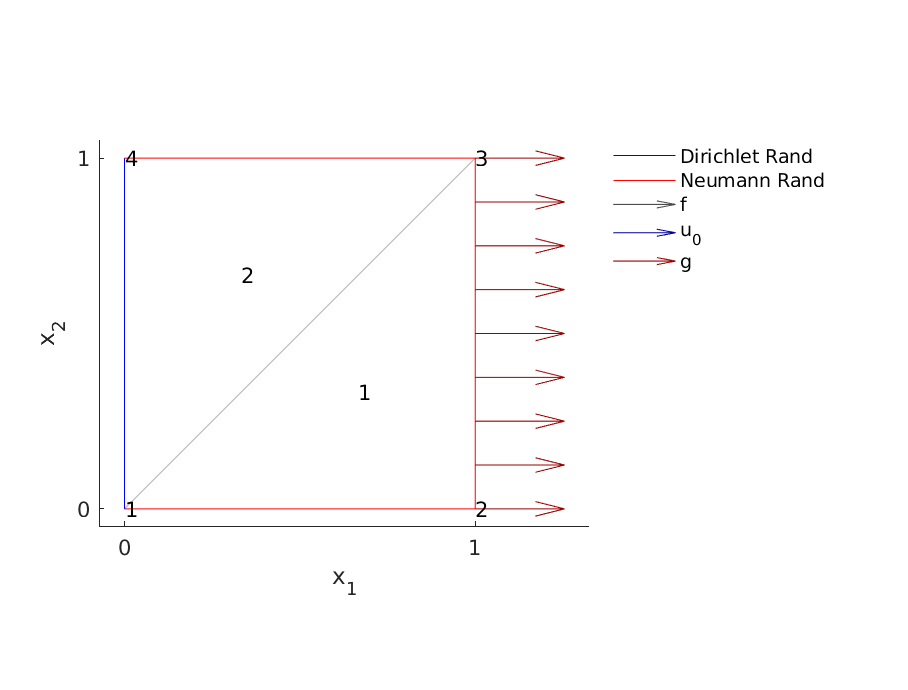
\includegraphics[width=\textwidth]{Plots/PullBoxInitial2}
	    \vspace*{-1.4cm}
	    \caption{Anfangskonfiguration}
	\end{figure}
\end{frame}

\begin{frame}
	\begin{figure}[h]
	    \centering
	    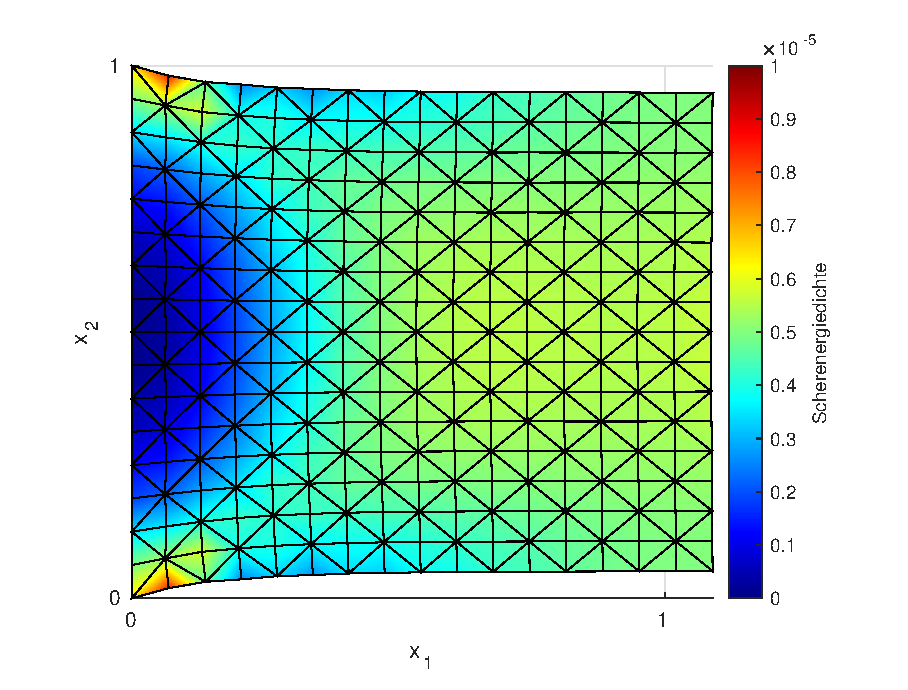
\includegraphics[width=\textwidth]{Plots/PullBoxUniformDeform3}
	    \caption{Numerische Lösung auf dem Gebiet.}
	\end{figure}
\end{frame}

\begin{frame}
	Fragen, die man sich stellen kann
	\begin{itemize}
		\item 
		Wie kann ich den Fehler der berechneten Lösung abschätzen, ohne die genaue Lösung zu kennen? $\rightarrow$ Fehlerschätzer
		\item
		Wie kann ich die Kenntnis über diesen Fehler gewinnbringend verwenden? $\rightarrow$ adaptive Gitterverfeinerung
	\end{itemize}
\end{frame}

\begin{frame}
	\begin{figure}[h]
	    \centering
	    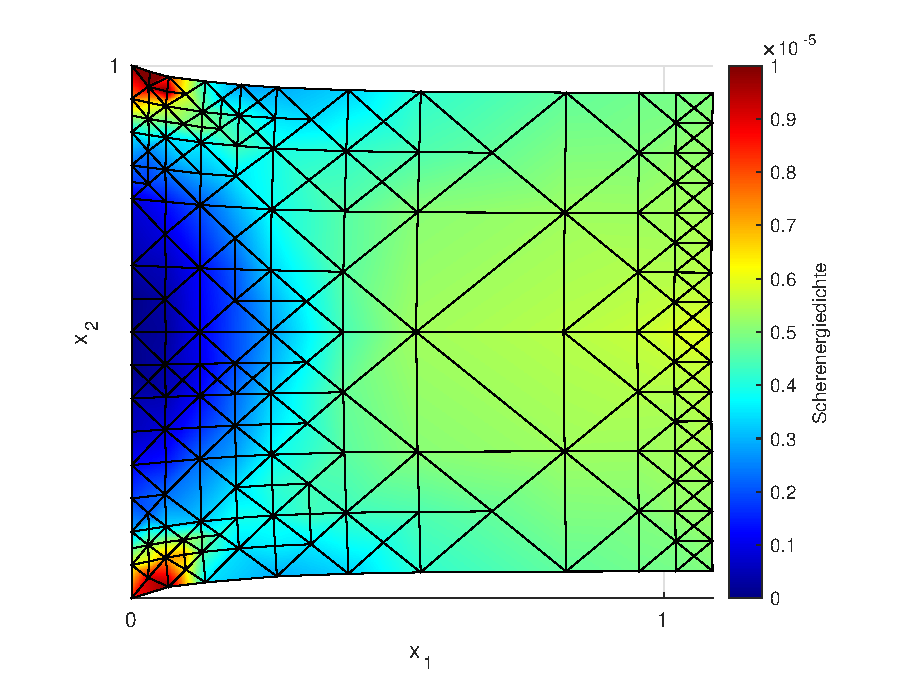
\includegraphics[width=\textwidth]{Plots/PullBoxAdaptiveDeform3}
	    \caption{Lösung mit adaptiven Methoden}
	\end{figure}
\end{frame}


\section{Formulierung des kontinuierlichen Problems}
\subsection*{Verschiebung und Spannungstensor}
\begin{frame}
	\frametitle{Formulierung des kontinuierlichen Problems}
	\begin{minipage}[t]{0.55\textwidth}
	Wir nehmen an, der Körper nimmt in Referenzkonfiguration das Gebiet $\overline{\Omega}\subseteq\R^d$ ein. Wir bezeichnen
	\begin{itemize}
		\item Deformation: Eine Abbildung $\chi\colon\overline{\Omega}\to\R^d$ mit $\det\nabla\chi>0$
		\item Verschiebung: Eine Abbildung $u$, gegeben durch $\chi=\Id+u$
	\end{itemize}
	Die Menge an zulässigen Verschiebungen bezeichnen wir mit $V$.
	\end{minipage}
	\hfill
	\begin{minipage}[t]{0.4\textwidth}
	\begin{figure}
	\centering
	\scalebox{0.7}{
	\input{Drawings/DefinitionVerschiebung1.pdf_tex}
	}
	\caption{Eine Deformation in 2D}
	\end{figure}
	\end{minipage}
\end{frame}

\begin{frame}
	Vorraussetzung des Models: Der deformierte Körper nimmt den Raum $\Omega$ ein und befindet sich im Kräftegleichgewicht. Man definiert
	\begin{minipage}[h]{0.6\textwidth}
	\vspace*{0.3cm}
	\begin{itemize}
	\item Volumenkräfte: Eine Abbildung $f\colon\Omega\to\R^d$.
	\item Oberflächenkräfte: Eine Abbildung $\sigma\colon\Omega\to\R^{d\times d}$ (Cauchyscher Spannungstensor). $\sigma_{ij}$ bezeichnet die Kraft auf die Fläche j in Richtung i wirkt. Kraft, die auf Oberfläche in Richtung $n$ wirkt ist
	\begin{align*}
		\sigma n =\sum_j\sigma_{ij}n_je_i\,.
	\end{align*}
	\end{itemize}
	\end{minipage}
	\hfill
	\begin{minipage}[h]{0.35\textwidth}
	\begin{figure}[h]
	\centering
	\scalebox{0.7}{
    \def\svgwidth{1.5\textwidth}
	\input{Drawings/SpannungstensorDarstellung.pdf_tex}
	}
	\caption{Darstellung eines Spannungstensors in 3D.}
	\end{figure}
	\end{minipage}
\end{frame}

\subsection*{Randbedingungen}
\begin{frame}
	\frametitle{Randbedingungen}
	Wir bezeichnen $\Gamma\coloneqq \partial\Omega$ als den Rand des Gebietes, $\Gamma_D\subseteq\Gamma$ als den Dirichlet- und $\Gamma_N\subseteq\Gamma$ als den Neumann-Rand. Damit erhalten wir Randbedingungen an die Lösung $u$ des Problems
	\begin{align*}
		\sigma n&= g &&\text{auf }\Gamma_N\,, \\
		u &= w &&\text{auf }\Gamma_D\,.
	\end{align*}
	mit $w\colon\Gamma_N\to\R^d$. Die Dirichlet-Randbedingung
	lässt sich verallgemeinern zu gleitenden Randbedingungen
	\begin{align*}
		Mu &= w &\text{ auf }\Gamma
	\end{align*}
	mit $M\colon\Gamma\to\R^{d\times d}$.
\end{frame}

\subsection*{Formulierung als Kräftegleichgewicht}
\begin{frame}
	\frametitle{Formulierung als Kräftegleichgewicht}
	Das Kräftegleichgewicht liefert die Formulierung: Finde eine Deformation $u$, so dass
	\vspace{1.5cm}
	\begin{align*}
		-\int_{\partial\omega}\tikzmark{forcesurf}{\sigma n}\dif s&=\int_\omega \tikzmark{forcevol}{f}\dif x &&\text{für alle }\omega\subseteq\Omega\text{ regulär genug}\,, \\
		\sigma n&= g &&\text{auf }\Gamma_N\,, \\
		Mu &= w &&\text{auf }\Gamma\,,
	\end{align*}
	\begin{tikzpicture}[remember picture, overlay, node distance = 1cm]
		\node[,text width=2.8cm] (forcevoldescr) [above right=0.8cm and 1.5cm of forcevol ]{Volumenkräfte, die auf $\omega$ wirken};
		\draw[,->,thick] (forcevoldescr) to [in=90,out=-90] (forcevol);
		\node[,text width=5cm] (forcesurfdescr) [above left=0.8cm and -3.5cm of forcesurf ]{Oberflächenkräfte, die über die Oberfläche $\partial\omega$ auf $\omega$ wirken};
		\draw[,->,thick] (forcesurfdescr) to [in=90,out=-90] (forcesurf);
	\end{tikzpicture}%
	wobei $\sigma$ von $u$ abhängt und $f,g$ als von $u$ unabhängig angenommen werden (tote Lasten). 
\end{frame}
%
%\begin{frame}
%	\begin{figure}[h]
%	\centering
%	% Graphic for TeX using PGF
% Title: /mnt/12CCB7B3CCB79009/Filing/Education/University/Bonn/Courses/Bachelorarbeit/Resources/BoundaryConditions1.dia
% Creator: Dia v0.97+git
% CreationDate: Mon Apr  4 20:43:29 2022
% For: theo
% \usepackage{tikz}
% The following commands are not supported in PSTricks at present
% We define them conditionally, so when they are implemented,
% this pgf file will use them.
\ifx\du\undefined
  \newlength{\du}
\fi
\setlength{\du}{15\unitlength}
\begin{tikzpicture}[even odd rule]
\pgftransformxscale{0.500000}
\pgftransformyscale{-0.500000}
\definecolor{dialinecolor}{rgb}{0.000000, 0.000000, 0.000000}
\pgfsetstrokecolor{dialinecolor}
\pgfsetstrokeopacity{1.000000}
\definecolor{diafillcolor}{rgb}{1.000000, 1.000000, 1.000000}
\pgfsetfillcolor{diafillcolor}
\pgfsetfillopacity{1.000000}
\pgfsetlinewidth{0.100000\du}
\pgfsetdash{}{0pt}
\pgfsetbuttcap
{
\definecolor{diafillcolor}{rgb}{0.000000, 0.000000, 0.000000}
\pgfsetfillcolor{diafillcolor}
\pgfsetfillopacity{1.000000}
% was here!!!
\definecolor{dialinecolor}{rgb}{0.000000, 0.000000, 0.000000}
\pgfsetstrokecolor{dialinecolor}
\pgfsetstrokeopacity{1.000000}
\draw (0.000000\du,0.000000\du)--(0.000000\du,-10.000000\du);
}
\pgfsetlinewidth{0.100000\du}
\pgfsetdash{}{0pt}
\pgfsetbuttcap
{
\definecolor{diafillcolor}{rgb}{0.000000, 0.000000, 0.000000}
\pgfsetfillcolor{diafillcolor}
\pgfsetfillopacity{1.000000}
% was here!!!
\definecolor{dialinecolor}{rgb}{0.000000, 0.000000, 0.000000}
\pgfsetstrokecolor{dialinecolor}
\pgfsetstrokeopacity{1.000000}
\draw (0.000000\du,-8.000000\du)--(17.000000\du,-8.000000\du);
}
\pgfsetlinewidth{0.100000\du}
\pgfsetdash{}{0pt}
\pgfsetbuttcap
{
\definecolor{diafillcolor}{rgb}{0.000000, 0.000000, 0.000000}
\pgfsetfillcolor{diafillcolor}
\pgfsetfillopacity{1.000000}
% was here!!!
\definecolor{dialinecolor}{rgb}{0.000000, 0.000000, 0.000000}
\pgfsetstrokecolor{dialinecolor}
\pgfsetstrokeopacity{1.000000}
\draw (17.000000\du,-8.000000\du)--(17.000000\du,-2.000000\du);
}
\pgfsetlinewidth{0.100000\du}
\pgfsetdash{}{0pt}
\pgfsetbuttcap
{
\definecolor{diafillcolor}{rgb}{0.000000, 0.000000, 0.000000}
\pgfsetfillcolor{diafillcolor}
\pgfsetfillopacity{1.000000}
% was here!!!
\definecolor{dialinecolor}{rgb}{0.000000, 0.000000, 0.000000}
\pgfsetstrokecolor{dialinecolor}
\pgfsetstrokeopacity{1.000000}
\draw (17.000000\du,-2.000000\du)--(0.000000\du,-2.000000\du);
}
\pgfsetlinewidth{0.100000\du}
\pgfsetdash{}{0pt}
\pgfsetbuttcap
{
\definecolor{diafillcolor}{rgb}{0.000000, 0.000000, 0.000000}
\pgfsetfillcolor{diafillcolor}
\pgfsetfillopacity{1.000000}
% was here!!!
\definecolor{dialinecolor}{rgb}{0.000000, 0.000000, 0.000000}
\pgfsetstrokecolor{dialinecolor}
\pgfsetstrokeopacity{1.000000}
\draw (0.000000\du,-10.000000\du)--(-1.000000\du,-9.000000\du);
}
\pgfsetlinewidth{0.100000\du}
\pgfsetdash{}{0pt}
\pgfsetbuttcap
{
\definecolor{diafillcolor}{rgb}{0.000000, 0.000000, 0.000000}
\pgfsetfillcolor{diafillcolor}
\pgfsetfillopacity{1.000000}
% was here!!!
\definecolor{dialinecolor}{rgb}{0.000000, 0.000000, 0.000000}
\pgfsetstrokecolor{dialinecolor}
\pgfsetstrokeopacity{1.000000}
\draw (0.000000\du,-8.000000\du)--(-1.000000\du,-7.000000\du);
}
\pgfsetlinewidth{0.100000\du}
\pgfsetdash{}{0pt}
\pgfsetbuttcap
{
\definecolor{diafillcolor}{rgb}{0.000000, 0.000000, 0.000000}
\pgfsetfillcolor{diafillcolor}
\pgfsetfillopacity{1.000000}
% was here!!!
\definecolor{dialinecolor}{rgb}{0.000000, 0.000000, 0.000000}
\pgfsetstrokecolor{dialinecolor}
\pgfsetstrokeopacity{1.000000}
\draw (0.000000\du,-6.000000\du)--(-1.000000\du,-5.000000\du);
}
\pgfsetlinewidth{0.100000\du}
\pgfsetdash{}{0pt}
\pgfsetbuttcap
{
\definecolor{diafillcolor}{rgb}{0.000000, 0.000000, 0.000000}
\pgfsetfillcolor{diafillcolor}
\pgfsetfillopacity{1.000000}
% was here!!!
\definecolor{dialinecolor}{rgb}{0.000000, 0.000000, 0.000000}
\pgfsetstrokecolor{dialinecolor}
\pgfsetstrokeopacity{1.000000}
\draw (0.000000\du,-4.000000\du)--(-1.000000\du,-3.000000\du);
}
\pgfsetlinewidth{0.100000\du}
\pgfsetdash{}{0pt}
\pgfsetbuttcap
{
\definecolor{diafillcolor}{rgb}{0.000000, 0.000000, 0.000000}
\pgfsetfillcolor{diafillcolor}
\pgfsetfillopacity{1.000000}
% was here!!!
\definecolor{dialinecolor}{rgb}{0.000000, 0.000000, 0.000000}
\pgfsetstrokecolor{dialinecolor}
\pgfsetstrokeopacity{1.000000}
\draw (0.000000\du,-2.000000\du)--(-1.000000\du,-1.000000\du);
}
\pgfsetlinewidth{0.100000\du}
\pgfsetdash{}{0pt}
\pgfsetbuttcap
{
\definecolor{diafillcolor}{rgb}{0.000000, 0.000000, 0.000000}
\pgfsetfillcolor{diafillcolor}
\pgfsetfillopacity{1.000000}
% was here!!!
\definecolor{dialinecolor}{rgb}{0.000000, 0.000000, 0.000000}
\pgfsetstrokecolor{dialinecolor}
\pgfsetstrokeopacity{1.000000}
\draw (0.000000\du,-9.000000\du)--(-1.000000\du,-8.000000\du);
}
\pgfsetlinewidth{0.100000\du}
\pgfsetdash{}{0pt}
\pgfsetbuttcap
{
\definecolor{diafillcolor}{rgb}{0.000000, 0.000000, 0.000000}
\pgfsetfillcolor{diafillcolor}
\pgfsetfillopacity{1.000000}
% was here!!!
\definecolor{dialinecolor}{rgb}{0.000000, 0.000000, 0.000000}
\pgfsetstrokecolor{dialinecolor}
\pgfsetstrokeopacity{1.000000}
\draw (0.000000\du,-7.000000\du)--(-1.000000\du,-6.000000\du);
}
\pgfsetlinewidth{0.100000\du}
\pgfsetdash{}{0pt}
\pgfsetbuttcap
{
\definecolor{diafillcolor}{rgb}{0.000000, 0.000000, 0.000000}
\pgfsetfillcolor{diafillcolor}
\pgfsetfillopacity{1.000000}
% was here!!!
\definecolor{dialinecolor}{rgb}{0.000000, 0.000000, 0.000000}
\pgfsetstrokecolor{dialinecolor}
\pgfsetstrokeopacity{1.000000}
\draw (0.000000\du,-5.000000\du)--(-1.000000\du,-4.000000\du);
}
\pgfsetlinewidth{0.100000\du}
\pgfsetdash{}{0pt}
\pgfsetbuttcap
{
\definecolor{diafillcolor}{rgb}{0.000000, 0.000000, 0.000000}
\pgfsetfillcolor{diafillcolor}
\pgfsetfillopacity{1.000000}
% was here!!!
\definecolor{dialinecolor}{rgb}{0.000000, 0.000000, 0.000000}
\pgfsetstrokecolor{dialinecolor}
\pgfsetstrokeopacity{1.000000}
\draw (0.000000\du,-3.000000\du)--(-1.000000\du,-2.000000\du);
}
\pgfsetlinewidth{0.100000\du}
\pgfsetdash{}{0pt}
\pgfsetbuttcap
{
\definecolor{diafillcolor}{rgb}{0.000000, 0.000000, 0.000000}
\pgfsetfillcolor{diafillcolor}
\pgfsetfillopacity{1.000000}
% was here!!!
\definecolor{dialinecolor}{rgb}{0.000000, 0.000000, 0.000000}
\pgfsetstrokecolor{dialinecolor}
\pgfsetstrokeopacity{1.000000}
\draw (0.000000\du,-1.000000\du)--(-1.000000\du,0.000000\du);
}
\pgfsetlinewidth{0.050000\du}
\pgfsetdash{}{0pt}
\pgfsetbuttcap
\definecolor{dialinecolor}{rgb}{0.000000, 0.000000, 0.000000}
\pgfsetstrokecolor{dialinecolor}
\pgfsetstrokeopacity{1.000000}
\pgfpathmoveto{\pgfpoint{17.192160\du}{-6.872710\du}}
\pgfpatharc{279}{270}{111.660170\du and 111.660170\du}
\pgfusepath{stroke}
\pgfsetlinewidth{0.050000\du}
\pgfsetdash{}{0pt}
\pgfsetbuttcap
\definecolor{dialinecolor}{rgb}{0.000000, 0.000000, 0.000000}
\pgfsetstrokecolor{dialinecolor}
\pgfsetstrokeopacity{1.000000}
\pgfpathmoveto{\pgfpoint{16.482919\du}{-0.929491\du}}
\pgfpatharc{279}{269}{94.994418\du and 94.994418\du}
\pgfusepath{stroke}
\pgfsetlinewidth{0.050000\du}
\pgfsetdash{}{0pt}
\pgfsetbuttcap
{
\definecolor{diafillcolor}{rgb}{0.000000, 0.000000, 0.000000}
\pgfsetfillcolor{diafillcolor}
\pgfsetfillopacity{1.000000}
% was here!!!
\definecolor{dialinecolor}{rgb}{0.000000, 0.000000, 0.000000}
\pgfsetstrokecolor{dialinecolor}
\pgfsetstrokeopacity{1.000000}
\draw (17.162252\du,-6.845827\du)--(16.453423\du,-0.936648\du);
}
\pgfsetlinewidth{0.100000\du}
\pgfsetdash{}{0pt}
\pgfsetbuttcap
{
\definecolor{diafillcolor}{rgb}{0.000000, 0.000000, 0.000000}
\pgfsetfillcolor{diafillcolor}
\pgfsetfillopacity{1.000000}
% was here!!!
\pgfsetarrowsend{to}
\definecolor{dialinecolor}{rgb}{0.000000, 0.000000, 0.000000}
\pgfsetstrokecolor{dialinecolor}
\pgfsetstrokeopacity{1.000000}
\draw (12.500000\du,-12.500000\du)--(12.500000\du,-8.000000\du);
}
% setfont left to latex
\definecolor{dialinecolor}{rgb}{0.000000, 0.000000, 0.000000}
\pgfsetstrokecolor{dialinecolor}
\pgfsetstrokeopacity{1.000000}
\definecolor{diafillcolor}{rgb}{0.000000, 0.000000, 0.000000}
\pgfsetfillcolor{diafillcolor}
\pgfsetfillopacity{1.000000}
\node[anchor=base west,inner sep=0pt,outer sep=0pt,color=dialinecolor] at (7.000000\du,-4.500000\du){$\Omega$};
% setfont left to latex
\definecolor{dialinecolor}{rgb}{0.000000, 0.000000, 0.000000}
\pgfsetstrokecolor{dialinecolor}
\pgfsetstrokeopacity{1.000000}
\definecolor{diafillcolor}{rgb}{0.000000, 0.000000, 0.000000}
\pgfsetfillcolor{diafillcolor}
\pgfsetfillopacity{1.000000}
\node[anchor=base west,inner sep=0pt,outer sep=0pt,color=dialinecolor] at (0.500000\du,-4.500000\du){$\Gamma_D$};
% setfont left to latex
\definecolor{dialinecolor}{rgb}{0.000000, 0.000000, 0.000000}
\pgfsetstrokecolor{dialinecolor}
\pgfsetstrokeopacity{1.000000}
\definecolor{diafillcolor}{rgb}{0.000000, 0.000000, 0.000000}
\pgfsetfillcolor{diafillcolor}
\pgfsetfillopacity{1.000000}
\node[anchor=base west,inner sep=0pt,outer sep=0pt,color=dialinecolor] at (6.081788\du,-8.609051\du){$\Gamma_N$};
% setfont left to latex
\definecolor{dialinecolor}{rgb}{0.000000, 0.000000, 0.000000}
\pgfsetstrokecolor{dialinecolor}
\pgfsetstrokeopacity{1.000000}
\definecolor{diafillcolor}{rgb}{0.000000, 0.000000, 0.000000}
\pgfsetfillcolor{diafillcolor}
\pgfsetfillopacity{1.000000}
\node[anchor=base west,inner sep=0pt,outer sep=0pt,color=dialinecolor] at (13.245364\du,-8.718101\du){$g$};
\end{tikzpicture}

%	\caption{Beispiel für mögliche Nebenbedingungen}
%	\end{figure}
%\end{frame}



\subsection*{Differenzielle Formulierung}
%\begin{frame}
%	Satz von Gauss liefert für $\omega\subseteq\Omega$
%	\begin{align*}
%		0 &= \int_\omega f\dif x + \int_{\partial\omega}\sigma\cdot n\dif s \\
%		&= \int_{\omega}f\dif x+\int_{\partial\omega}\sum_j\sigma_{ij}n_je_i\dif s \\
%		&= \int_{\omega}f+\sum_j\partial_j\sigma_{ij}e_i\dif x
%	\end{align*}
%	
%	mit $n\colon\Omega\to\R^d$ die Flächennormale.
%	Wir erhalten die Gleichgewichtsbeziehung in differenzieller Form
%	\begin{align*}
%		-\diver \sigma \coloneqq -\sum_j\partial_j\sigma_{ij}e_i =f
%	\end{align*}
%\end{frame}

\begin{frame}
	\frametitle{Differenzielle Formulierung}
%	Es folgt, wenn wir annehmen, dass $\sigma_{ij}$ in $j$ differenzierbar ist
%	\begin{align*}
%		\int_\omega f\dif x &=  -\int_{\partial\omega}\sigma n\dif s \\
%		&= -\int_{\partial\omega}\sum_{i,j}\sigma_{ij}n_je_i\dif s \\
%		&\tikzmark{gaussglw}{=} -\int_{\omega}\sum_{i,j}\partial_j\sigma_{ij}e_i\dif x
%	\end{align*}
%	\begin{tikzpicture}[remember picture, overlay, node distance = 0.6cm]
%		\node[,text width=5cm] (gaussglwdescr) [below right= of gaussglw]{Satz von Gauss};
%		\draw[,->,thick] (gaussglwdescr) to [in=-90,out=180] (gaussglw);
%	\end{tikzpicture}
%	\vspace{0.5cm}
	Der Satz von Gauss liefert
	\begin{align*}
		-\diver \sigma \coloneqq -\sum_j\partial_j\sigma_{ij}e_i =f
	\end{align*}
	Jetzt haben wir die differenzielle Formulierung
	\begin{align*}
		\qquad\qquad-\diver\sigma &= f &&\text{auf }\Omega\,,\qquad\qquad\\
		\sigma n &= g &&\text{auf }\Gamma_N\,, \\
		Mu &= w &&\text{auf }\Gamma\,.
	\end{align*}
\end{frame}

\subsection*{Materialgesetze}
\subsubsection*{Hooke-Tensor}
\begin{frame}
	\frametitle{Materialgesetze}
	Das Ziel ist es einen Ausdruck für $\sigma$ in Abhängigkeit von $u$ zu erhalten.
	Wir definieren den linearisierten Verzerrungstensor
	\begin{align*}
		\e\coloneqq\frac{1}{2}\left(\nabla u+\nabla u^\top\right)\,.
	\end{align*}
	Für ein linear-elastisches Material ist
	\begin{align*}
		\sigma_{ij}=\sum_{k,l}C_{ijkl}\e_{kl}
	\end{align*}
	mit Hooke-Tensor $C\colon\Omega\to\bigotimes_{i=1}^4\R^d$. 
%	Die Impulserhaltung liefert die Symmetrie $\sigma_{ij}=\sigma_{ji}$. Damit erhält man
%	\begin{align*}
%		C_{ijkl} = C_{jikl}
%	\end{align*}
%	Wir fordern weiter die Symmetriebeziehung
%	\begin{align*}
%		C_{ijkl} = C_{klij}
%	\end{align*}
\end{frame}

\subsubsection*{St. Venant-Kirchhoff Material}
\begin{frame}
	Für St. Venant-Kirchhoff-Materialen gilt
	\begin{align*}
		C_{ijkl}=\lambda\delta_{ij}\delta_{kl}+\mu(\delta_{ik}\delta_{jl}+\delta_{il}\delta_{jk})
	\end{align*}
	mit Lamé-Koeffizienten $\lambda$ und $\mu$. Es folgt
	\begin{align*}
		\sigma_{ij}=\sum_{k,l}C_{ijkl}\e_{kl}=\lambda\Tr(\e)\delta_{ij}+2\mu\e_{ij}\,.
	\end{align*}
\end{frame}

%\subsection*{Implementierung des Hooke Tensors}
%\begin{frame}[allowframebreaks]
%	\frametitle{Implementierung des Hooke Tensors}
%	
%	Wir wenden die Voigt representation für $d=2$
%	\begin{align*}
%		\gamma(\e) = \vect{\e_{11} \\ \e_{22} \\ 2\e_{12}}
%	\end{align*}
%	beziehungsweise für $d=3$ an
%	\begin{align*}
%		\gamma(\e) = \vect{\e_{11} \\ \e_{22} \\ \e_{22} \\ 2\e_{12} \\ 2\e_{13} \\ 2\e_{23}}
%	\end{align*}
%	
%	\framebreak
%	Damit lässt sich die Relation 
%	\begin{align*}
%		\sigma_{ij}=\sum_{k,l}C_{ijkl}\e_{kl}=\lambda\Tr(\e)\delta_{ij}+2\mu\e_{ij}
%	\end{align*}
%	schreiben als
%	\begin{align*}
%		\vect{\sigma_{11} \\ \sigma_{22} \\ \sigma_{33} \\ \sigma_{12} \\ \sigma_{13} \\ \sigma_{23}}
%		= \underbrace{\begin{pmatrix}
%			\lambda+2\mu & \lambda & \lambda & & & \\
%			\lambda & \lambda+2\mu & \lambda & & & \\
%			\lambda & \lambda & \lambda+2\mu & & & \\
%			& & & \mu & & \\
%			& & & & \mu & \\
%			& & & & & \mu \\
%		\end{pmatrix}}_{\eqqcolon \hC}
%		\vect{\e_{11} \\ \e_{22} \\ \e_{33} \\ 2\e_{12} \\ 2\e_{13} \\ 2\e_{23}}
%	\end{align*}
%	also $\gamma(\sigma) = \hC\gamma(\e)$
%\end{frame}

%\begin{frame}
%	Für St. Venant-Kirchhoff-Materialien ergibt sich die Lamé-Differenzialgleichung
%	\begin{align*}
%		-\lambda\nabla\diver u-2\mu\diver\e(u)&=f &&\text{auf }\Omega\qquad \\
%		Mu &= w &&\text{auf }\Gamma \\
%		\sigma n &= g &&\text{auf }\Gamma_N
%	\end{align*}
%\end{frame}


\subsection*{Variationelle Formulierung}

%\begin{frame}
%	\frametitle{Variationsmethode, Energiebetrachtungen}
%	 Wir betrachten die Arbeit, die Verrichtet wird, wenn wir das Objekt im Endzustand $u$ um ein kleines $v\in V^0$ verschieben:
%	\begin{align*}
%		&\int_{\Gamma_N}g\cdot v\dif s+\int_\Omega f\cdot v\dif x\\
%		&= \int_{\partial\Omega}(\sigma(u)\, n)\cdot v\dif s+\int_\Omega \sum_if_iv_i\dif x \\
%		&= \int_{\partial\Omega}\sum_{i,j}\sigma_{ij}v_in_j\dif s - \int_\Omega \sum_{i,j}(\partial_j\sigma_{ij})v_i\dif x \\
%		&= \int_{\Omega}\sum_{i,j}\partial_j\left(\sigma_{ij}v_i\right)\dif x -\int_\Omega \sum_{i,j}(\partial_j\sigma_{ij})v_i\dif x \\
%		&= \int_\Omega \sum_{i,j}\sigma_{ij}(\partial_jv_i)\dif x \\
%	\end{align*}
%\end{frame}
%
%\begin{frame}
%	Und weiter
%	\begin{align*}
%		&\int_{\Gamma_N}g\cdot v\dif s+\int_\Omega f\cdot v\dif x\\
%		&= \int_\Omega \sum_{i,j}\sigma_{ij}(\partial_jv_i)\dif x \\
%		&= \int_\Omega \sum_{i,j}\sigma_{ij}\frac{1}{2}(\partial_jv_i+\partial_iv_j)\dif x \\
%		&= \int_\Omega \sum_{i,j}\sigma_{ij}(u)\e_{ij}(v)\dif x \\
%	\end{align*}
%\end{frame}

\begin{frame}
	\frametitle{Variationelle Formulierung}
	Wir setzen nun $V\coloneqq H^1(\Omega;\R^d)$ als die Menge der möglichen Verschiebungen. Außerdem definieren wir
	\begin{align*}
		V^0\coloneqq\{v\in H^1(\Omega;\R^d)\colon Mv = 0 \text{ auf }\Gamma\}\,.
	\end{align*}
	Wir definieren
	\begin{align*}
		a(u,v) \coloneqq\int_\Omega\sigma(u):\e(v)\dif x \coloneqq\int_\Omega \sum_{i,j}\sigma_{ij}(u)\e_{ij}(v)\dif x
	\end{align*}
	sowie
	\begin{align*}
		\ell(v)\coloneqq
		\inner{f,v}_{0,\Omega}+\inner{g,v}_{0,\Gamma_N}
		=\int_\Omega f\cdot v\dif x+\int_{\Gamma_N}g\cdot v \dif s\,.
	\end{align*}
\end{frame}

\begin{frame}
	Man kann aus der differenziellen Formulierungen eine variationelle Formulierung (virtuelle Arbeit) herleiten: 
	Finde $u\in V$, so dass
	\begin{align*}
		a(u,v)&= \ell(v) \qquad &&\text{für alle }v\in V^0\,,\qquad\\
		Mu &= w &&\text{auf }\Gamma\,.
	\end{align*}
\end{frame}

\subsection*{Energiebetrachtung}
\begin{frame}
	\frametitle{Energiebetrachtung}
	Wir erhalten für die potenzielle Energie des Zustandes $v$
	\begin{align*}
		W(v)\coloneqq \frac{1}{2}a(v,v)-\ell(v)\,.
	\end{align*}
	Man kann eine Formulierung als Optimierungsproblem herleiten:
	Finde $u\in V$, so dass
	\begin{equation*}
		\begin{aligned}
			u\text{ minimiert }&&  &W=\frac{1}{2}a(\cdot,\cdot)-\ell\,, \\
		\text{unter der Nebenbedingung }&&  &Mu\big\vert_\Gamma = w\big\vert_\Gamma\,.
		\end{aligned}
	\end{equation*}
\end{frame}


\section{Existenz und Eindeutigkeit des kontinuierlichen Problems}
\subsection*{Lax-Milgram-Lemma}

\begin{frame}
	\frametitle{Existenz und Eindeutigkeit des kontinuierlichen Problems}
	Das folgende Resultat findet sich in \cite[S.288]{Cia-1988}.
	\begin{theorem}[Lax-Milgram Lemma]\label{th:LaxMilgramLemma}
		Seien $V^0$ ein Banach-Raum, $\ell\colon V^0\to\R$ eine stetige lineare Form und $a\colon V^0\times V^0\to\R$ eine stetige symmetrische elliptische bilineare Form.
		Dann hat das Problem $u\in V^0$ zu finden, so dass
		\begin{align*}
			a(u,v)=\ell(v)
		\end{align*}
		für alle $v\in V^0$, eine eindeutige Lösung. Dieses ist dann auch eindeutige Lösung des Problems $u\in V^0$ zu finden, so dass $u$ das Funktional
		\begin{align*}
			W=\frac{1}{2}a(\cdot,\cdot)-\ell
		\end{align*}
		minimiert.
	\end{theorem}
\end{frame}

\begin{frame}
	\frametitle{Existenz und Eindeutigkeit des inhomogenen Problems}
	\begin{corollary}
		Existiert $u_\Gamma\in V$, so dass $Mu_\Gamma=w$ und erfüllen $a$ und $\ell$ die Vorraussetzung des Lax-Milgram-Lemmas auf $V^0$, dann besitzt unser Problem eine Eindeutige Lösung.
	\end{corollary}
	\begin{proof}
		Es ist $u\in V$ genau dann eine Lösung von 
		\begin{align*}
			a(u,v)&= \ell(v) \qquad &&\text{für alle }v\in V^0\,,\qquad\\
			Mu &= w &&\text{auf }\Gamma\,,
		\end{align*}
		wenn $u-u_\Gamma\in V^0$ eine Lösung ist von
		\begin{align*}
			a(u-u_\Gamma,v)&= \ell(v)-a(u_\Gamma,v) \qquad &&\text{für alle }v\in V^0\,.
		\end{align*}
	\end{proof}
\end{frame}

\begin{frame}
	Es ist recht einfach zu zeigen, dass
	\begin{itemize}
		\item $a$ ist bilinear und symmetrisch.
		\item Stetigkeit: Es gibt ein $c_A>0$, so dass für alle $v_1,v_2\in V$
		\begin{align*}
			a(v_1,v_2)\leq c_A\norm{v_1}\norm{v_2}\,.
		\end{align*}
	\end{itemize}
	Es ist nicht sehr einfach zu zeigen, dass
	\begin{itemize}
		\item Elliptizität: Es gibt ein $c_a>0$, so dass für alle $v\in V$
		\begin{align*}
			a(v,v)\geq c_a\norm{v}^2\,.
		\end{align*}
	\end{itemize}
\end{frame}

\begin{frame}
	\begin{figure}[h]
	\centering
	\hspace*{-0.4cm}
	% Graphic for TeX using PGF
% Title: /mnt/12CCB7B3CCB79009/Filing/Education/University/Bonn/Courses/Bachelorarbeit/Resources/UniquenessFlowchart2.dia
% Creator: Dia v0.97+git
% CreationDate: Mon May 23 18:17:04 2022
% For: theo
% \usepackage{tikz}
% The following commands are not supported in PSTricks at present
% We define them conditionally, so when they are implemented,
% this pgf file will use them.
\ifx\du\undefined
  \newlength{\du}
\fi
\setlength{\du}{15\unitlength}
\begin{tikzpicture}[even odd rule]
\pgftransformxscale{1.000000}
\pgftransformyscale{-1.000000}
\definecolor{dialinecolor}{rgb}{0.000000, 0.000000, 0.000000}
\pgfsetstrokecolor{dialinecolor}
\pgfsetstrokeopacity{1.000000}
\definecolor{diafillcolor}{rgb}{1.000000, 1.000000, 1.000000}
\pgfsetfillcolor{diafillcolor}
\pgfsetfillopacity{1.000000}
\pgfsetlinewidth{0.050000\du}
\pgfsetdash{}{0pt}
\pgfsetmiterjoin
{\pgfsetcornersarced{\pgfpoint{0.000000\du}{0.000000\du}}\definecolor{diafillcolor}{rgb}{1.000000, 1.000000, 1.000000}
\pgfsetfillcolor{diafillcolor}
\pgfsetfillopacity{1.000000}
\fill (11.546250\du,-7.182420\du)--(11.546250\du,-5.332420\du)--(19.156250\du,-5.332420\du)--(19.156250\du,-7.182420\du)--cycle;
}{\pgfsetcornersarced{\pgfpoint{0.000000\du}{0.000000\du}}\definecolor{dialinecolor}{rgb}{0.000000, 0.000000, 0.000000}
\pgfsetstrokecolor{dialinecolor}
\pgfsetstrokeopacity{1.000000}
\draw (11.546250\du,-7.182420\du)--(11.546250\du,-5.332420\du)--(19.156250\du,-5.332420\du)--(19.156250\du,-7.182420\du)--cycle;
}% setfont left to latex
\definecolor{dialinecolor}{rgb}{0.000000, 0.000000, 0.000000}
\pgfsetstrokecolor{dialinecolor}
\pgfsetstrokeopacity{1.000000}
\definecolor{diafillcolor}{rgb}{0.000000, 0.000000, 0.000000}
\pgfsetfillcolor{diafillcolor}
\pgfsetfillopacity{1.000000}
\node[anchor=base,inner sep=0pt, outer sep=0pt,color=dialinecolor] at (15.351250\du,-6.063357\du){Lax-Milgram-Lemma};
\pgfsetlinewidth{0.050000\du}
\pgfsetdash{}{0pt}
\pgfsetmiterjoin
{\pgfsetcornersarced{\pgfpoint{0.000000\du}{0.000000\du}}\definecolor{diafillcolor}{rgb}{1.000000, 1.000000, 1.000000}
\pgfsetfillcolor{diafillcolor}
\pgfsetfillopacity{1.000000}
\fill (12.248750\du,-10.225000\du)--(12.248750\du,-8.375000\du)--(18.451250\du,-8.375000\du)--(18.451250\du,-10.225000\du)--cycle;
}{\pgfsetcornersarced{\pgfpoint{0.000000\du}{0.000000\du}}\definecolor{dialinecolor}{rgb}{0.000000, 0.000000, 0.000000}
\pgfsetstrokecolor{dialinecolor}
\pgfsetstrokeopacity{1.000000}
\draw (12.248750\du,-10.225000\du)--(12.248750\du,-8.375000\du)--(18.451250\du,-8.375000\du)--(18.451250\du,-10.225000\du)--cycle;
}% setfont left to latex
\definecolor{dialinecolor}{rgb}{0.000000, 0.000000, 0.000000}
\pgfsetstrokecolor{dialinecolor}
\pgfsetstrokeopacity{1.000000}
\definecolor{diafillcolor}{rgb}{0.000000, 0.000000, 0.000000}
\pgfsetfillcolor{diafillcolor}
\pgfsetfillopacity{1.000000}
\node[anchor=base,inner sep=0pt, outer sep=0pt,color=dialinecolor] at (15.350000\du,-9.105937\du){Elliptizität von a};
\pgfsetlinewidth{0.050000\du}
\pgfsetdash{}{0pt}
\pgfsetmiterjoin
{\pgfsetcornersarced{\pgfpoint{0.000000\du}{0.000000\du}}\definecolor{diafillcolor}{rgb}{1.000000, 1.000000, 1.000000}
\pgfsetfillcolor{diafillcolor}
\pgfsetfillopacity{1.000000}
\fill (11.260000\du,-14.175000\du)--(11.260000\du,-11.525000\du)--(19.440000\du,-11.525000\du)--(19.440000\du,-14.175000\du)--cycle;
}{\pgfsetcornersarced{\pgfpoint{0.000000\du}{0.000000\du}}\definecolor{dialinecolor}{rgb}{0.000000, 0.000000, 0.000000}
\pgfsetstrokecolor{dialinecolor}
\pgfsetstrokeopacity{1.000000}
\draw (11.260000\du,-14.175000\du)--(11.260000\du,-11.525000\du)--(19.440000\du,-11.525000\du)--(19.440000\du,-14.175000\du)--cycle;
}% setfont left to latex
\definecolor{dialinecolor}{rgb}{0.000000, 0.000000, 0.000000}
\pgfsetstrokecolor{dialinecolor}
\pgfsetstrokeopacity{1.000000}
\definecolor{diafillcolor}{rgb}{0.000000, 0.000000, 0.000000}
\pgfsetfillcolor{diafillcolor}
\pgfsetfillopacity{1.000000}
\node[anchor=base,inner sep=0pt, outer sep=0pt,color=dialinecolor] at (15.350000\du,-13.055938\du){Kornsche Ungleichung};
% setfont left to latex
\definecolor{dialinecolor}{rgb}{0.000000, 0.000000, 0.000000}
\pgfsetstrokecolor{dialinecolor}
\pgfsetstrokeopacity{1.000000}
\definecolor{diafillcolor}{rgb}{0.000000, 0.000000, 0.000000}
\pgfsetfillcolor{diafillcolor}
\pgfsetfillopacity{1.000000}
\node[anchor=base,inner sep=0pt, outer sep=0pt,color=dialinecolor] at (15.350000\du,-12.255937\du){mit Ranbedingungen};
\pgfsetlinewidth{0.050000\du}
\pgfsetdash{}{0pt}
\pgfsetmiterjoin
{\pgfsetcornersarced{\pgfpoint{0.000000\du}{0.000000\du}}\definecolor{diafillcolor}{rgb}{1.000000, 1.000000, 1.000000}
\pgfsetfillcolor{diafillcolor}
\pgfsetfillopacity{1.000000}
\fill (5.058750\du,-11.875000\du)--(5.058750\du,-8.425000\du)--(10.241250\du,-8.425000\du)--(10.241250\du,-11.875000\du)--cycle;
}{\pgfsetcornersarced{\pgfpoint{0.000000\du}{0.000000\du}}\definecolor{dialinecolor}{rgb}{0.000000, 0.000000, 0.000000}
\pgfsetstrokecolor{dialinecolor}
\pgfsetstrokeopacity{1.000000}
\draw (5.058750\du,-11.875000\du)--(5.058750\du,-8.425000\du)--(10.241250\du,-8.425000\du)--(10.241250\du,-11.875000\du)--cycle;
}% setfont left to latex
\definecolor{dialinecolor}{rgb}{0.000000, 0.000000, 0.000000}
\pgfsetstrokecolor{dialinecolor}
\pgfsetstrokeopacity{1.000000}
\definecolor{diafillcolor}{rgb}{0.000000, 0.000000, 0.000000}
\pgfsetfillcolor{diafillcolor}
\pgfsetfillopacity{1.000000}
\node[anchor=base,inner sep=0pt, outer sep=0pt,color=dialinecolor] at (7.650000\du,-10.755937\du){a stetig,};
% setfont left to latex
\definecolor{dialinecolor}{rgb}{0.000000, 0.000000, 0.000000}
\pgfsetstrokecolor{dialinecolor}
\pgfsetstrokeopacity{1.000000}
\definecolor{diafillcolor}{rgb}{0.000000, 0.000000, 0.000000}
\pgfsetfillcolor{diafillcolor}
\pgfsetfillopacity{1.000000}
\node[anchor=base,inner sep=0pt, outer sep=0pt,color=dialinecolor] at (7.650000\du,-9.955937\du){symmetrisch};
% setfont left to latex
\definecolor{dialinecolor}{rgb}{0.000000, 0.000000, 0.000000}
\pgfsetstrokecolor{dialinecolor}
\pgfsetstrokeopacity{1.000000}
\definecolor{diafillcolor}{rgb}{0.000000, 0.000000, 0.000000}
\pgfsetfillcolor{diafillcolor}
\pgfsetfillopacity{1.000000}
\node[anchor=base,inner sep=0pt, outer sep=0pt,color=dialinecolor] at (7.650000\du,-9.155937\du){und bilinear};
\pgfsetlinewidth{0.050000\du}
\pgfsetdash{}{0pt}
\pgfsetmiterjoin
{\pgfsetcornersarced{\pgfpoint{0.000000\du}{0.000000\du}}\definecolor{diafillcolor}{rgb}{1.000000, 1.000000, 1.000000}
\pgfsetfillcolor{diafillcolor}
\pgfsetfillopacity{1.000000}
\fill (5.683750\du,-4.033790\du)--(5.683750\du,-2.183790\du)--(25.061250\du,-2.183790\du)--(25.061250\du,-4.033790\du)--cycle;
}{\pgfsetcornersarced{\pgfpoint{0.000000\du}{0.000000\du}}\definecolor{dialinecolor}{rgb}{0.000000, 0.000000, 0.000000}
\pgfsetstrokecolor{dialinecolor}
\pgfsetstrokeopacity{1.000000}
\draw (5.683750\du,-4.033790\du)--(5.683750\du,-2.183790\du)--(25.061250\du,-2.183790\du)--(25.061250\du,-4.033790\du)--cycle;
}% setfont left to latex
\definecolor{dialinecolor}{rgb}{0.000000, 0.000000, 0.000000}
\pgfsetstrokecolor{dialinecolor}
\pgfsetstrokeopacity{1.000000}
\definecolor{diafillcolor}{rgb}{0.000000, 0.000000, 0.000000}
\pgfsetfillcolor{diafillcolor}
\pgfsetfillopacity{1.000000}
\node[anchor=base,inner sep=0pt, outer sep=0pt,color=dialinecolor] at (15.372500\du,-2.914727\du){Existenz und Eindeutigkeit des kontinuierlichen Problems};
\pgfsetlinewidth{0.050000\du}
\pgfsetdash{}{0pt}
\pgfsetmiterjoin
{\pgfsetcornersarced{\pgfpoint{0.000000\du}{0.000000\du}}\definecolor{diafillcolor}{rgb}{1.000000, 1.000000, 1.000000}
\pgfsetfillcolor{diafillcolor}
\pgfsetfillopacity{1.000000}
\fill (20.277850\du,-11.075000\du)--(20.277850\du,-8.425000\du)--(27.180350\du,-8.425000\du)--(27.180350\du,-11.075000\du)--cycle;
}{\pgfsetcornersarced{\pgfpoint{0.000000\du}{0.000000\du}}\definecolor{dialinecolor}{rgb}{0.000000, 0.000000, 0.000000}
\pgfsetstrokecolor{dialinecolor}
\pgfsetstrokeopacity{1.000000}
\draw (20.277850\du,-11.075000\du)--(20.277850\du,-8.425000\du)--(27.180350\du,-8.425000\du)--(27.180350\du,-11.075000\du)--cycle;
}% setfont left to latex
\definecolor{dialinecolor}{rgb}{0.000000, 0.000000, 0.000000}
\pgfsetstrokecolor{dialinecolor}
\pgfsetstrokeopacity{1.000000}
\definecolor{diafillcolor}{rgb}{0.000000, 0.000000, 0.000000}
\pgfsetfillcolor{diafillcolor}
\pgfsetfillopacity{1.000000}
\node[anchor=base,inner sep=0pt, outer sep=0pt,color=dialinecolor] at (23.729100\du,-9.955937\du){Randbedingungen};
% setfont left to latex
\definecolor{dialinecolor}{rgb}{0.000000, 0.000000, 0.000000}
\pgfsetstrokecolor{dialinecolor}
\pgfsetstrokeopacity{1.000000}
\definecolor{diafillcolor}{rgb}{0.000000, 0.000000, 0.000000}
\pgfsetfillcolor{diafillcolor}
\pgfsetfillopacity{1.000000}
\node[anchor=base,inner sep=0pt, outer sep=0pt,color=dialinecolor] at (23.729100\du,-9.155937\du){erfüllbar, l stetig};
\pgfsetlinewidth{0.050000\du}
\pgfsetdash{}{0pt}
\pgfsetbuttcap
{
\definecolor{diafillcolor}{rgb}{0.000000, 0.000000, 0.000000}
\pgfsetfillcolor{diafillcolor}
\pgfsetfillopacity{1.000000}
% was here!!!
\pgfsetarrowsend{latex}
\definecolor{dialinecolor}{rgb}{0.000000, 0.000000, 0.000000}
\pgfsetstrokecolor{dialinecolor}
\pgfsetstrokeopacity{1.000000}
\draw (15.350000\du,-8.375000\du)--(15.351300\du,-7.182420\du);
}
\pgfsetlinewidth{0.050000\du}
\pgfsetdash{}{0pt}
\pgfsetbuttcap
{
\definecolor{diafillcolor}{rgb}{0.000000, 0.000000, 0.000000}
\pgfsetfillcolor{diafillcolor}
\pgfsetfillopacity{1.000000}
% was here!!!
\pgfsetarrowsend{latex}
\definecolor{dialinecolor}{rgb}{0.000000, 0.000000, 0.000000}
\pgfsetstrokecolor{dialinecolor}
\pgfsetstrokeopacity{1.000000}
\draw (15.351300\du,-5.332420\du)--(15.372500\du,-4.033790\du);
}
\pgfsetlinewidth{0.050000\du}
\pgfsetdash{}{0pt}
\pgfsetbuttcap
{
\definecolor{diafillcolor}{rgb}{0.000000, 0.000000, 0.000000}
\pgfsetfillcolor{diafillcolor}
\pgfsetfillopacity{1.000000}
% was here!!!
\pgfsetarrowsend{latex}
\definecolor{dialinecolor}{rgb}{0.000000, 0.000000, 0.000000}
\pgfsetstrokecolor{dialinecolor}
\pgfsetstrokeopacity{1.000000}
\draw (23.729100\du,-8.425000\du)--(15.351300\du,-7.182420\du);
}
\pgfsetlinewidth{0.050000\du}
\pgfsetdash{}{0pt}
\pgfsetbuttcap
{
\definecolor{diafillcolor}{rgb}{0.000000, 0.000000, 0.000000}
\pgfsetfillcolor{diafillcolor}
\pgfsetfillopacity{1.000000}
% was here!!!
\pgfsetarrowsend{latex}
\definecolor{dialinecolor}{rgb}{0.000000, 0.000000, 0.000000}
\pgfsetstrokecolor{dialinecolor}
\pgfsetstrokeopacity{1.000000}
\draw (7.650000\du,-8.425000\du)--(15.351300\du,-7.182420\du);
}
\pgfsetlinewidth{0.050000\du}
\pgfsetdash{}{0pt}
\pgfsetbuttcap
{
\definecolor{diafillcolor}{rgb}{0.000000, 0.000000, 0.000000}
\pgfsetfillcolor{diafillcolor}
\pgfsetfillopacity{1.000000}
% was here!!!
\pgfsetarrowsend{latex}
\definecolor{dialinecolor}{rgb}{0.000000, 0.000000, 0.000000}
\pgfsetstrokecolor{dialinecolor}
\pgfsetstrokeopacity{1.000000}
\draw (15.350000\du,-11.525000\du)--(15.350000\du,-10.225000\du);
}
\end{tikzpicture}

	\end{figure}
\end{frame}


\subsection*{Kornsche Ungleichung ohne Randbedingungen}

\subsubsection*{Kornsche Ungleichung ohne Randbedingungen auf dem Ganzraum}
\begin{frame}
	\frametitle{Kornsche Ungleichungen}
	Man definiert für $v\in H^1(\Omega;\R^d)$ die Norm
	\begin{align*}
		\norm{v}_{K,\Omega}^2\coloneqq\norm{v}_{0,\Omega}^2+\norm{\e(v)}_{0,\Omega}^2\,.
	\end{align*}
	Da $\e\colon H^1(\Omega;\R^d)\to H^0(\Omega;\R^d)$ linear ist, folgt 1-Homogenität und die Dreiecksungleichung. Die Positivdefinitheit auf dem Ganzraum folgt aus folgendem Resultat in \cite[S.292]{Bra-2007}:
	\begin{lemma}[Kornsche Ungleichung ohne Randbedingungen auf dem Ganzraum]
	Sei $\Omega=\R^d$ mit $v\in H^1(\Omega;\R^d)$. Dann gilt
	\begin{align*}
		\abs{v}_{1,\Omega}\leq\sqrt{2}\norm{\e(v)}_{0,\Omega}\,.
	\end{align*}
	\end{lemma}
\end{frame}

\subsubsection*{Kornsche Ungleichung ohne Randbedingungen auf C1-Mengen}
\begin{frame}
	\begin{lemma}[Kornsche Ungleichung ohne Randbedingungen auf $C^1$-Mengen]
	Sei $\Omega\subseteq\R^d$ eine $C^1$-Menge, dann gibt es ein $c_{K1}>0$, so dass für alle $v\in H^1(\Omega;\R^d)$ gilt
	\begin{align*}
		\norm{v}_{1,\Omega}\leq c_{K1}\norm{v}_{K,\Omega}\,.
	\end{align*}
	\end{lemma}
\end{frame}

\begin{frame}
	\begin{proof}
	Siehe \cite{Nit-1981} für Details.
	\begin{figure}[h]
	\centering
	% Graphic for TeX using PGF
% Title: /mnt/12CCB7B3CCB79009/Filing/Education/University/Bonn/Courses/Bachelorarbeit/PraesentationBegleitseminar/Drawings/KornFlowchart1.dia
% Creator: Dia v0.97+git
% CreationDate: Fri Jul 29 09:25:20 2022
% For: theo
% \usepackage{tikz}
% The following commands are not supported in PSTricks at present
% We define them conditionally, so when they are implemented,
% this pgf file will use them.
\ifx\du\undefined
  \newlength{\du}
\fi
\setlength{\du}{15\unitlength}
\begin{tikzpicture}[even odd rule]
\pgftransformxscale{1.000000}
\pgftransformyscale{-1.000000}
\definecolor{dialinecolor}{rgb}{0.000000, 0.000000, 0.000000}
\pgfsetstrokecolor{dialinecolor}
\pgfsetstrokeopacity{1.000000}
\definecolor{diafillcolor}{rgb}{1.000000, 1.000000, 1.000000}
\pgfsetfillcolor{diafillcolor}
\pgfsetfillopacity{1.000000}
\pgfsetlinewidth{0.050000\du}
\pgfsetdash{}{0pt}
\pgfsetmiterjoin
{\pgfsetcornersarced{\pgfpoint{0.000000\du}{0.000000\du}}\definecolor{diafillcolor}{rgb}{1.000000, 1.000000, 1.000000}
\pgfsetfillcolor{diafillcolor}
\pgfsetfillopacity{1.000000}
\fill (-9.096570\du,-3.335480\du)--(-9.096570\du,0.114520\du)--(-0.916570\du,0.114520\du)--(-0.916570\du,-3.335480\du)--cycle;
}{\pgfsetcornersarced{\pgfpoint{0.000000\du}{0.000000\du}}\definecolor{dialinecolor}{rgb}{0.000000, 0.000000, 0.000000}
\pgfsetstrokecolor{dialinecolor}
\pgfsetstrokeopacity{1.000000}
\draw (-9.096570\du,-3.335480\du)--(-9.096570\du,0.114520\du)--(-0.916570\du,0.114520\du)--(-0.916570\du,-3.335480\du)--cycle;
}% setfont left to latex
\definecolor{dialinecolor}{rgb}{0.000000, 0.000000, 0.000000}
\pgfsetstrokecolor{dialinecolor}
\pgfsetstrokeopacity{1.000000}
\definecolor{diafillcolor}{rgb}{0.000000, 0.000000, 0.000000}
\pgfsetfillcolor{diafillcolor}
\pgfsetfillopacity{1.000000}
\node[anchor=base,inner sep=0pt, outer sep=0pt,color=dialinecolor] at (-5.006570\du,-2.216418\du){Kornsche Ungleichung};
% setfont left to latex
\definecolor{dialinecolor}{rgb}{0.000000, 0.000000, 0.000000}
\pgfsetstrokecolor{dialinecolor}
\pgfsetstrokeopacity{1.000000}
\definecolor{diafillcolor}{rgb}{0.000000, 0.000000, 0.000000}
\pgfsetfillcolor{diafillcolor}
\pgfsetfillopacity{1.000000}
\node[anchor=base,inner sep=0pt, outer sep=0pt,color=dialinecolor] at (-5.006570\du,-1.416418\du){ohne Randbedingung};
% setfont left to latex
\definecolor{dialinecolor}{rgb}{0.000000, 0.000000, 0.000000}
\pgfsetstrokecolor{dialinecolor}
\pgfsetstrokeopacity{1.000000}
\definecolor{diafillcolor}{rgb}{0.000000, 0.000000, 0.000000}
\pgfsetfillcolor{diafillcolor}
\pgfsetfillopacity{1.000000}
\node[anchor=base,inner sep=0pt, outer sep=0pt,color=dialinecolor] at (-5.006570\du,-0.616418\du){auf dem Ganzraum};
\pgfsetlinewidth{0.050000\du}
\pgfsetdash{}{0pt}
\pgfsetmiterjoin
{\pgfsetcornersarced{\pgfpoint{0.000000\du}{0.000000\du}}\definecolor{diafillcolor}{rgb}{1.000000, 1.000000, 1.000000}
\pgfsetfillcolor{diafillcolor}
\pgfsetfillopacity{1.000000}
\fill (-3.491458\du,-7.401467\du)--(-3.491458\du,-4.751467\du)--(9.098542\du,-4.751467\du)--(9.098542\du,-7.401467\du)--cycle;
}{\pgfsetcornersarced{\pgfpoint{0.000000\du}{0.000000\du}}\definecolor{dialinecolor}{rgb}{0.000000, 0.000000, 0.000000}
\pgfsetstrokecolor{dialinecolor}
\pgfsetstrokeopacity{1.000000}
\draw (-3.491458\du,-7.401467\du)--(-3.491458\du,-4.751467\du)--(9.098542\du,-4.751467\du)--(9.098542\du,-7.401467\du)--cycle;
}% setfont left to latex
\definecolor{dialinecolor}{rgb}{0.000000, 0.000000, 0.000000}
\pgfsetstrokecolor{dialinecolor}
\pgfsetstrokeopacity{1.000000}
\definecolor{diafillcolor}{rgb}{0.000000, 0.000000, 0.000000}
\pgfsetfillcolor{diafillcolor}
\pgfsetfillopacity{1.000000}
\node[anchor=base,inner sep=0pt, outer sep=0pt,color=dialinecolor] at (2.803542\du,-6.282405\du){Konstruktion einer Erweiterung von };
% setfont left to latex
\definecolor{dialinecolor}{rgb}{0.000000, 0.000000, 0.000000}
\pgfsetstrokecolor{dialinecolor}
\pgfsetstrokeopacity{1.000000}
\definecolor{diafillcolor}{rgb}{0.000000, 0.000000, 0.000000}
\pgfsetfillcolor{diafillcolor}
\pgfsetfillopacity{1.000000}
\node[anchor=base,inner sep=0pt, outer sep=0pt,color=dialinecolor] at (2.803542\du,-5.482405\du){Epigraphen auf den Ganzraum};
\pgfsetlinewidth{0.050000\du}
\pgfsetdash{}{0pt}
\pgfsetmiterjoin
{\pgfsetcornersarced{\pgfpoint{0.000000\du}{0.000000\du}}\definecolor{diafillcolor}{rgb}{1.000000, 1.000000, 1.000000}
\pgfsetfillcolor{diafillcolor}
\pgfsetfillopacity{1.000000}
\fill (-9.131540\du,-7.377150\du)--(-9.131540\du,-4.727150\du)--(-4.789040\du,-4.727150\du)--(-4.789040\du,-7.377150\du)--cycle;
}{\pgfsetcornersarced{\pgfpoint{0.000000\du}{0.000000\du}}\definecolor{dialinecolor}{rgb}{0.000000, 0.000000, 0.000000}
\pgfsetstrokecolor{dialinecolor}
\pgfsetstrokeopacity{1.000000}
\draw (-9.131540\du,-7.377150\du)--(-9.131540\du,-4.727150\du)--(-4.789040\du,-4.727150\du)--(-4.789040\du,-7.377150\du)--cycle;
}% setfont left to latex
\definecolor{dialinecolor}{rgb}{0.000000, 0.000000, 0.000000}
\pgfsetstrokecolor{dialinecolor}
\pgfsetstrokeopacity{1.000000}
\definecolor{diafillcolor}{rgb}{0.000000, 0.000000, 0.000000}
\pgfsetfillcolor{diafillcolor}
\pgfsetfillopacity{1.000000}
\node[anchor=base,inner sep=0pt, outer sep=0pt,color=dialinecolor] at (-6.960290\du,-6.258088\du){Zerlegung};
% setfont left to latex
\definecolor{dialinecolor}{rgb}{0.000000, 0.000000, 0.000000}
\pgfsetstrokecolor{dialinecolor}
\pgfsetstrokeopacity{1.000000}
\definecolor{diafillcolor}{rgb}{0.000000, 0.000000, 0.000000}
\pgfsetfillcolor{diafillcolor}
\pgfsetfillopacity{1.000000}
\node[anchor=base,inner sep=0pt, outer sep=0pt,color=dialinecolor] at (-6.960290\du,-5.458088\du){der Eins};
\pgfsetlinewidth{0.050000\du}
\pgfsetdash{}{0pt}
\pgfsetmiterjoin
{\pgfsetcornersarced{\pgfpoint{0.000000\du}{0.000000\du}}\definecolor{diafillcolor}{rgb}{1.000000, 1.000000, 1.000000}
\pgfsetfillcolor{diafillcolor}
\pgfsetfillopacity{1.000000}
\fill (0.423451\du,-3.335480\du)--(0.423451\du,0.114520\du)--(9.125951\du,0.114520\du)--(9.125951\du,-3.335480\du)--cycle;
}{\pgfsetcornersarced{\pgfpoint{0.000000\du}{0.000000\du}}\definecolor{dialinecolor}{rgb}{0.000000, 0.000000, 0.000000}
\pgfsetstrokecolor{dialinecolor}
\pgfsetstrokeopacity{1.000000}
\draw (0.423451\du,-3.335480\du)--(0.423451\du,0.114520\du)--(9.125951\du,0.114520\du)--(9.125951\du,-3.335480\du)--cycle;
}% setfont left to latex
\definecolor{dialinecolor}{rgb}{0.000000, 0.000000, 0.000000}
\pgfsetstrokecolor{dialinecolor}
\pgfsetstrokeopacity{1.000000}
\definecolor{diafillcolor}{rgb}{0.000000, 0.000000, 0.000000}
\pgfsetfillcolor{diafillcolor}
\pgfsetfillopacity{1.000000}
\node[anchor=base,inner sep=0pt, outer sep=0pt,color=dialinecolor] at (4.774701\du,-2.216418\du){Kornsche Ungleichung};
% setfont left to latex
\definecolor{dialinecolor}{rgb}{0.000000, 0.000000, 0.000000}
\pgfsetstrokecolor{dialinecolor}
\pgfsetstrokeopacity{1.000000}
\definecolor{diafillcolor}{rgb}{0.000000, 0.000000, 0.000000}
\pgfsetfillcolor{diafillcolor}
\pgfsetfillopacity{1.000000}
\node[anchor=base,inner sep=0pt, outer sep=0pt,color=dialinecolor] at (4.774701\du,-1.416418\du){ohne Randbedingungen};
% setfont left to latex
\definecolor{dialinecolor}{rgb}{0.000000, 0.000000, 0.000000}
\pgfsetstrokecolor{dialinecolor}
\pgfsetstrokeopacity{1.000000}
\definecolor{diafillcolor}{rgb}{0.000000, 0.000000, 0.000000}
\pgfsetfillcolor{diafillcolor}
\pgfsetfillopacity{1.000000}
\node[anchor=base,inner sep=0pt, outer sep=0pt,color=dialinecolor] at (4.774701\du,-0.616418\du){auf $C^1$-Mengen};
\pgfsetlinewidth{0.050000\du}
\pgfsetdash{}{0pt}
\pgfsetbuttcap
{
\definecolor{diafillcolor}{rgb}{0.000000, 0.000000, 0.000000}
\pgfsetfillcolor{diafillcolor}
\pgfsetfillopacity{1.000000}
% was here!!!
\pgfsetarrowsend{latex}
\definecolor{dialinecolor}{rgb}{0.000000, 0.000000, 0.000000}
\pgfsetstrokecolor{dialinecolor}
\pgfsetstrokeopacity{1.000000}
\draw (-0.921569\du,-1.610480\du)--(0.423451\du,-1.610480\du);
}
\pgfsetlinewidth{0.050000\du}
\pgfsetdash{}{0pt}
\pgfsetbuttcap
{
\definecolor{diafillcolor}{rgb}{0.000000, 0.000000, 0.000000}
\pgfsetfillcolor{diafillcolor}
\pgfsetfillopacity{1.000000}
% was here!!!
\pgfsetarrowsend{latex}
\definecolor{dialinecolor}{rgb}{0.000000, 0.000000, 0.000000}
\pgfsetstrokecolor{dialinecolor}
\pgfsetstrokeopacity{1.000000}
\draw (4.767154\du,-4.075465\du)--(4.774701\du,-3.335480\du);
}
\pgfsetlinewidth{0.050000\du}
\pgfsetdash{}{0pt}
\pgfsetbuttcap
{
\definecolor{diafillcolor}{rgb}{0.000000, 0.000000, 0.000000}
\pgfsetfillcolor{diafillcolor}
\pgfsetfillopacity{1.000000}
% was here!!!
\definecolor{dialinecolor}{rgb}{0.000000, 0.000000, 0.000000}
\pgfsetstrokecolor{dialinecolor}
\pgfsetstrokeopacity{1.000000}
\draw (-6.960290\du,-4.727150\du)--(-6.956989\du,-4.067360\du);
}
\pgfsetlinewidth{0.050000\du}
\pgfsetdash{}{0pt}
\pgfsetbuttcap
{
\definecolor{diafillcolor}{rgb}{0.000000, 0.000000, 0.000000}
\pgfsetfillcolor{diafillcolor}
\pgfsetfillopacity{1.000000}
% was here!!!
\definecolor{dialinecolor}{rgb}{0.000000, 0.000000, 0.000000}
\pgfsetstrokecolor{dialinecolor}
\pgfsetstrokeopacity{1.000000}
\draw (-6.965094\du,-4.071412\du)--(4.767154\du,-4.071412\du);
}
\pgfsetlinewidth{0.050000\du}
\pgfsetdash{}{0pt}
\pgfsetbuttcap
{
\definecolor{diafillcolor}{rgb}{0.000000, 0.000000, 0.000000}
\pgfsetfillcolor{diafillcolor}
\pgfsetfillopacity{1.000000}
% was here!!!
\definecolor{dialinecolor}{rgb}{0.000000, 0.000000, 0.000000}
\pgfsetstrokecolor{dialinecolor}
\pgfsetstrokeopacity{1.000000}
\draw (2.803542\du,-4.751467\du)--(2.805700\du,-4.067360\du);
}
\end{tikzpicture}

%	\caption{Beweis durch Diagramm}
	\end{figure}
	\end{proof}
\end{frame}

%\begin{frame}
%	\begin{proof}
%		Wir rechnen
%		\begin{align*}
%			\norm{v}_{1,\Omega}^2
%			&\leq\norm{Ev}_{1,\R^d}^2 \\
%			&\leq\sqrt{2}\left(\abs{\e(Ev)}_{0,\R^d}^2+\abs{Ev}_{0,\R^d}^2\right) \\
%			&=\sqrt{2}\left(\sum_{i,j}\abs{\partial_i(Ev_j)+\partial_j(Ev_i)}_{0,\R^d}^2+\abs{Ev}_{0,\R^d}^2\right) \\
%			&\leq c_E\sqrt{2}\left(\sum_{i,j}\abs{\partial_i(v_j)+\partial_j(v_i)}_{0,\Omega}+\abs{v}_{0,\Omega}^2\right) \\
%			&= c_K\norm{v}_{K,\Omega}^2
%		\end{align*}
%	\end{proof}
%\end{frame}

\subsection*{Kornsche Ungleichung mit Randbedingungen}
%\begin{frame}
%	Wir bezeichnen eine offene zusammenhängende Menge $\Omega\subseteq\R^d$ als Gebiet.
%	\begin{lemma}[Eine Charakterisierung von Starrkörperbewegungen]
%		Sei $\Omega\subseteq\R^3$ ein Gebiet, dann sind für $v\in H^1(\Omega;\R^3)$ äquivalent
%		\begin{enumerate}
%			\item $\e(v) = 0$
%			\item Es gibt $a,b\in\R^3$, so dass $v(x)=a\times x+b$
%		\end{enumerate}
%	\end{lemma}
%\end{frame}

\begin{frame}
	Wir bezeichnen eine offene zusammenhängende Menge $\Omega\subseteq\R^d$ als Gebiet. Ein Gebiet mit $C^1$-Rand bezeichnen wir als $C^1$-Gebiet.
	\begin{theorem}[Kornsche Ungleichung mit Randbedingungen]
		Seien $\Omega\subseteq\R^3$ ein $C^1$-Gebiet und $S\subseteq\Gamma$ mit positivem Flächenmaß. Dann gibt es $c_{K2}>0$, so dass für alle $v\in H^1_{S}(\Omega;\R^3)$ gilt
		\begin{align*}
			\norm{v}_{1,\Omega}\leq c_{K2}\norm{\e(v)}_{0,\Omega}\,.
		\end{align*}
	\end{theorem}
\end{frame}


\begin{frame}
	\begin{proof}
	Siehe \cite[S.294f.]{Cia-1988} und \cite[S.293]{Bra-2007} für Details.
	\begin{figure}[h]
	\centering
	% Graphic for TeX using PGF
% Title: /mnt/12CCB7B3CCB79009/Filing/Education/University/Bonn/Courses/Bachelorarbeit/Resources/KornFlowchart2.dia
% Creator: Dia v0.97+git
% CreationDate: Mon May 23 18:17:35 2022
% For: theo
% \usepackage{tikz}
% The following commands are not supported in PSTricks at present
% We define them conditionally, so when they are implemented,
% this pgf file will use them.
\ifx\du\undefined
  \newlength{\du}
\fi
\setlength{\du}{15\unitlength}
\begin{tikzpicture}[even odd rule]
\pgftransformxscale{1.000000}
\pgftransformyscale{-1.000000}
\definecolor{dialinecolor}{rgb}{0.000000, 0.000000, 0.000000}
\pgfsetstrokecolor{dialinecolor}
\pgfsetstrokeopacity{1.000000}
\definecolor{diafillcolor}{rgb}{1.000000, 1.000000, 1.000000}
\pgfsetfillcolor{diafillcolor}
\pgfsetfillopacity{1.000000}
\pgfsetlinewidth{0.050000\du}
\pgfsetdash{}{0pt}
\pgfsetmiterjoin
{\pgfsetcornersarced{\pgfpoint{0.000000\du}{0.000000\du}}\definecolor{diafillcolor}{rgb}{1.000000, 1.000000, 1.000000}
\pgfsetfillcolor{diafillcolor}
\pgfsetfillopacity{1.000000}
\fill (1.000000\du,-4.845000\du)--(1.000000\du,-1.395000\du)--(9.702500\du,-1.395000\du)--(9.702500\du,-4.845000\du)--cycle;
}{\pgfsetcornersarced{\pgfpoint{0.000000\du}{0.000000\du}}\definecolor{dialinecolor}{rgb}{0.000000, 0.000000, 0.000000}
\pgfsetstrokecolor{dialinecolor}
\pgfsetstrokeopacity{1.000000}
\draw (1.000000\du,-4.845000\du)--(1.000000\du,-1.395000\du)--(9.702500\du,-1.395000\du)--(9.702500\du,-4.845000\du)--cycle;
}% setfont left to latex
\definecolor{dialinecolor}{rgb}{0.000000, 0.000000, 0.000000}
\pgfsetstrokecolor{dialinecolor}
\pgfsetstrokeopacity{1.000000}
\definecolor{diafillcolor}{rgb}{0.000000, 0.000000, 0.000000}
\pgfsetfillcolor{diafillcolor}
\pgfsetfillopacity{1.000000}
\node[anchor=base,inner sep=0pt, outer sep=0pt,color=dialinecolor] at (5.351250\du,-3.725937\du){Kornsche Ungleichung};
% setfont left to latex
\definecolor{dialinecolor}{rgb}{0.000000, 0.000000, 0.000000}
\pgfsetstrokecolor{dialinecolor}
\pgfsetstrokeopacity{1.000000}
\definecolor{diafillcolor}{rgb}{0.000000, 0.000000, 0.000000}
\pgfsetfillcolor{diafillcolor}
\pgfsetfillopacity{1.000000}
\node[anchor=base,inner sep=0pt, outer sep=0pt,color=dialinecolor] at (5.351250\du,-2.925937\du){ohne Randbedingungen};
% setfont left to latex
\definecolor{dialinecolor}{rgb}{0.000000, 0.000000, 0.000000}
\pgfsetstrokecolor{dialinecolor}
\pgfsetstrokeopacity{1.000000}
\definecolor{diafillcolor}{rgb}{0.000000, 0.000000, 0.000000}
\pgfsetfillcolor{diafillcolor}
\pgfsetfillopacity{1.000000}
\node[anchor=base,inner sep=0pt, outer sep=0pt,color=dialinecolor] at (5.351250\du,-2.125938\du){auf $C^1$-Mengen};
\pgfsetlinewidth{0.050000\du}
\pgfsetdash{}{0pt}
\pgfsetmiterjoin
{\pgfsetcornersarced{\pgfpoint{0.000000\du}{0.000000\du}}\definecolor{diafillcolor}{rgb}{1.000000, 1.000000, 1.000000}
\pgfsetfillcolor{diafillcolor}
\pgfsetfillopacity{1.000000}
\fill (11.486250\du,-8.375000\du)--(11.486250\du,-5.725000\du)--(20.313750\du,-5.725000\du)--(20.313750\du,-8.375000\du)--cycle;
}{\pgfsetcornersarced{\pgfpoint{0.000000\du}{0.000000\du}}\definecolor{dialinecolor}{rgb}{0.000000, 0.000000, 0.000000}
\pgfsetstrokecolor{dialinecolor}
\pgfsetstrokeopacity{1.000000}
\draw (11.486250\du,-8.375000\du)--(11.486250\du,-5.725000\du)--(20.313750\du,-5.725000\du)--(20.313750\du,-8.375000\du)--cycle;
}% setfont left to latex
\definecolor{dialinecolor}{rgb}{0.000000, 0.000000, 0.000000}
\pgfsetstrokecolor{dialinecolor}
\pgfsetstrokeopacity{1.000000}
\definecolor{diafillcolor}{rgb}{0.000000, 0.000000, 0.000000}
\pgfsetfillcolor{diafillcolor}
\pgfsetfillopacity{1.000000}
\node[anchor=base,inner sep=0pt, outer sep=0pt,color=dialinecolor] at (15.900000\du,-7.255937\du){Charakterisierung von };
% setfont left to latex
\definecolor{dialinecolor}{rgb}{0.000000, 0.000000, 0.000000}
\pgfsetstrokecolor{dialinecolor}
\pgfsetstrokeopacity{1.000000}
\definecolor{diafillcolor}{rgb}{0.000000, 0.000000, 0.000000}
\pgfsetfillcolor{diafillcolor}
\pgfsetfillopacity{1.000000}
\node[anchor=base,inner sep=0pt, outer sep=0pt,color=dialinecolor] at (15.900000\du,-6.455938\du){Starrkörperbewegungen};
\pgfsetlinewidth{0.050000\du}
\pgfsetdash{}{0pt}
\pgfsetmiterjoin
{\pgfsetcornersarced{\pgfpoint{0.000000\du}{0.000000\du}}\definecolor{diafillcolor}{rgb}{1.000000, 1.000000, 1.000000}
\pgfsetfillcolor{diafillcolor}
\pgfsetfillopacity{1.000000}
\fill (11.810000\du,-4.425000\du)--(11.810000\du,-1.775000\du)--(19.990000\du,-1.775000\du)--(19.990000\du,-4.425000\du)--cycle;
}{\pgfsetcornersarced{\pgfpoint{0.000000\du}{0.000000\du}}\definecolor{dialinecolor}{rgb}{0.000000, 0.000000, 0.000000}
\pgfsetstrokecolor{dialinecolor}
\pgfsetstrokeopacity{1.000000}
\draw (11.810000\du,-4.425000\du)--(11.810000\du,-1.775000\du)--(19.990000\du,-1.775000\du)--(19.990000\du,-4.425000\du)--cycle;
}% setfont left to latex
\definecolor{dialinecolor}{rgb}{0.000000, 0.000000, 0.000000}
\pgfsetstrokecolor{dialinecolor}
\pgfsetstrokeopacity{1.000000}
\definecolor{diafillcolor}{rgb}{0.000000, 0.000000, 0.000000}
\pgfsetfillcolor{diafillcolor}
\pgfsetfillopacity{1.000000}
\node[anchor=base,inner sep=0pt, outer sep=0pt,color=dialinecolor] at (15.900000\du,-3.305937\du){Kornsche Ungleichung};
% setfont left to latex
\definecolor{dialinecolor}{rgb}{0.000000, 0.000000, 0.000000}
\pgfsetstrokecolor{dialinecolor}
\pgfsetstrokeopacity{1.000000}
\definecolor{diafillcolor}{rgb}{0.000000, 0.000000, 0.000000}
\pgfsetfillcolor{diafillcolor}
\pgfsetfillopacity{1.000000}
\node[anchor=base,inner sep=0pt, outer sep=0pt,color=dialinecolor] at (15.900000\du,-2.505937\du){mit Randbedingungen};
\pgfsetlinewidth{0.050000\du}
\pgfsetdash{}{0pt}
\pgfsetbuttcap
{
\definecolor{diafillcolor}{rgb}{0.000000, 0.000000, 0.000000}
\pgfsetfillcolor{diafillcolor}
\pgfsetfillopacity{1.000000}
% was here!!!
\pgfsetarrowsend{latex}
\definecolor{dialinecolor}{rgb}{0.000000, 0.000000, 0.000000}
\pgfsetstrokecolor{dialinecolor}
\pgfsetstrokeopacity{1.000000}
\draw (9.692500\du,-3.120000\du)--(11.815000\du,-3.100000\du);
}
\pgfsetlinewidth{0.050000\du}
\pgfsetdash{}{0pt}
\pgfsetbuttcap
{
\definecolor{diafillcolor}{rgb}{0.000000, 0.000000, 0.000000}
\pgfsetfillcolor{diafillcolor}
\pgfsetfillopacity{1.000000}
% was here!!!
\pgfsetarrowsend{latex}
\definecolor{dialinecolor}{rgb}{0.000000, 0.000000, 0.000000}
\pgfsetstrokecolor{dialinecolor}
\pgfsetstrokeopacity{1.000000}
\draw (15.900000\du,-5.725000\du)--(15.900000\du,-4.425000\du);
}
\end{tikzpicture}

%	\caption{Beweis durch Diagramm}
	\end{figure}
	\end{proof}
\end{frame}

%\subsection*{Elliptizität von a}
%\begin{frame}
%	\begin{corollary}[Elliptizität von $a$]\label{pr:elliptizitaeta}
%		Sei $\Omega\subseteq\R^3$ ein Lipschitz-Gebiet und $C\in L^\infty(\Omega;\otimes_{i=1}^4\R^d)$ elliptisch, so ist $a\colon V\times V\to \R$ auch elliptisch, d.h. es gibt ein $c_a>0$, so dass für alle $v\in V$
%		\begin{align*}
%			a(v,v)\geq c_a\norm{v}^2
%		\end{align*}
%	\end{corollary}
%\end{frame}
%
%\begin{frame}
%	\begin{proof}
%		Die Kornsche Ungleichung mit Randbedingungen liefert
%		\begin{align*}
%			a(v,v)&=\int_\Omega\e(v):\sigma(v)\dif x \\
%			&= \int_\Omega\sum_{i,j,k,l}\e_{ij}(v)C_{ijkl}\e_{kl}(v)\dif x\dif x \\
%			&\geq c_c\int_\Omega\sum_{i,j}\e_{ij}(v)\e_{ij}(v)\dif x\dif x \\
%			&\geq c_a\norm{v}_{1,\Omega} \\
%		\end{align*}
%	\end{proof}
%\end{frame}


\section{Das diskrete Problem}
\subsection*{Triangulierungen}
\begin{frame}
	\frametitle{Triangulierungen}
	\begin{minipage}[h]{0.5\textwidth}
	Für eine reguläre Triangulierung $\cT$ von $\Omega$ definieren wir
	\begin{itemize}
		\item
		$\cE$ ist die Menge der Kanten
		\item
		$\cE_\Gamma = \cE_D\cup\cE_N$ ist die Menge der Rand-Kanten
		\item
		$\cK=\{x^i\}_{i=1}^n$ ist die Menge der Knoten
		\item
		$\cK_\Gamma = \cK_D\cup\cK_N = \{x^{i_j}\}_{j=1}^l$ ist die Menge der Rand-Knoten
	\end{itemize}
	\end{minipage}
	\hfill
	\begin{minipage}[h]{0.48\textwidth}
	\begin{figure}[h]
	\centering
	\scalebox{0.7}{
	\input{Drawings/Triangulation3.pdf_tex}
	}
	\caption{Beispiel einer Triangulierung}
	\end{figure}
	\end{minipage}
\end{frame}

\subsection*{Nodale Basis}
\begin{frame}
	\frametitle{Nodale Basis}
	Bezeichne $\varphi_i$ die nodale Basis in einer Dimension. Wir definieren die $d$-dimensionale nodale Basis
	\begin{align*}
		\vect{\phi_1\cdots\phi_{dn}}=\vect{\varphi_1\ev_1\cdots\varphi_1\ev_d\quad\cdots\quad \varphi_n\ev_1\cdots\varphi_n\ev_d}
	\end{align*}
	% Weiter setzen wir $\cS_h\coloneqq\Span\{\phi_i\}_i$.
	\begin{figure}[h]
	\centering
	\scalebox{0.7}{
	\input{Drawings/NodalBasis3.pdf_tex}
	}
	\caption{Ein Element einer nodalen Basis in 2D}
	\end{figure}
\end{frame}

\subsection*{Diskrete Formulierung}
\begin{frame}
	\frametitle{Diskrete Formulierung}
	Wir diskretisieren
	\begin{align*}
		&V=H^1(\Omega;\R^d) &&\longrightarrow V_h\coloneqq\Span\{\phi_i\}_i\subseteq V \\
		&V^0 = \{v\in H^1(\Omega;\R^d)\colon Mv = 0\text{ auf }\Gamma\} &&\longrightarrow
		V^0_h \coloneqq V_h\cap V^0
	\end{align*}
	und erhalten die diskrete Formulierung: Finde $u_h\in V_h$, so dass
	\begin{align*}
		\begin{aligned}
		a(u_h,v_h) &= \ell(v_h) &&\text{für alle }v_h\in V_h^0, \\
		Mu_h &= w &&\text{auf }\Gamma.
		\end{aligned}
	\end{align*}
\end{frame}
%
\section{A priori Fehlerabschätzung}
\begin{frame}
	\frametitle{A priori Fehlerabschätzung}
	Man definiert den Fehler
	\begin{align*}
		e\coloneqq u-u_h
	\end{align*}
	\begin{proposition}[A priori Fehler]
		Seien $\cT$ eine uniforme Triangulierung, $u\in H^2(\Omega;\R^2)$. Dann gibt ein $c>0$, welches vom Regularitätsparameter und $\Omega$ abhängt, so dass
		\begin{align*}
			\norm{e}_{1,\Omega}\leq c\frac{c_A}{c_a}h \abs{u}_{2,\Omega}\,.
		\end{align*}
		Hierbei ist $h\coloneqq\max_{T\in\cT}h_T$.
	\end{proposition}
	\begin{proof}
		Folgt aus Céa's Lemma in \cite[S.53]{Bra-2007} und einem Interpolationsresultat aus \cite[S.75]{Bra-2007}.
	\end{proof}
\end{frame}

%\begin{frame}
%	Sei $\Gamma_D>0$, dann ist $\abs{\cdot}_{1,\Omega}$ nach der Poincaré-Ungleichung auf $V$ eine Norm. Wir erhalten dann
%	\begin{lemma}[Céa's Lemma]
%		Der Approximationsfehler erfüllt
%		\begin{align*}
%			\abs{e}_{1,\Omega} \leq \frac{c_A}{c_a}\inf_{v_h\in V^0_h}\abs{u-v_h}_{1,\Omega}
%		\end{align*}
%	\end{lemma}
%	\begin{proof}
%		Siehe \cite{Ged-2021b}.
%	\end{proof}
%\end{frame}
%
%\begin{frame}
%	Das folgende Resultat ist aus \cite{Ged-2021b}
%	\begin{lemma}[Interpolation]
%		Sei $\cT$ eine reguläre Triangulierung. Dann gibt es einen Interpolationsoperator $I^T_h\colon V\to V_{0,h}$ und ein $c>0$, so dass für alle $v\in V^0$
%		\begin{align*}
%			\abs{v-I^T_hv}_{1,\Omega}\leq c_I h_\cT \abs{v}_{2,\Omega}
%		\end{align*}
%	\end{lemma}
%\end{frame}
%
%\begin{frame}
%	Insgesamt gibt es also eine von der Triangulierung unabhängige Konstante $c>0$, so dass
%	\begin{align*}
%		\abs{\e(e)}_{0,\Omega}
%		&= \abs{e}_{1,\Omega} \\
%		&\leq c \inf_{v_h\in V^0_h}\abs{u-v_h}_{1,\Omega} \\
%		&\leq c \abs{u-I^T_hv}_{1,\Omega} \\
%		&\leq c h_\cT \abs{v}_{2,\Omega}
%	\end{align*}
%\end{frame}

\section{A posteriori Fehlerschätzer}
\subsection*{Residualer Fehlerschätzer}
\begin{frame}
	\frametitle{Ein residualer Fehlerschätzer}
	Wir definieren
	\begin{itemize}
		\item die flächenbezogenen Residuen $R_T\coloneqq f+\diver\sigma(u_h)$
		\item die kantenbezogenen Sprünge
		\begin{align*}
			R_E \coloneqq \begin{cases}
				\left[\![\sigma(u_h)n_E\right]\!] &,\text{falls }E\in\cE\setminus\cE_\Gamma \\
				g-\sigma(u_h)n_E &,\text{falls }E\in\cE_N \\
				0 &,\text{sonst }
			\end{cases}
		\end{align*}
%		mit
%		\begin{align*}
%		\left[\![\sigma(u_h)\cdot n\right]\!]
%		&\coloneqq\sigma(u_h)\cdot n_{T_1}\big\Vert_{\partial T_1}+\sigma(u_h)\cdot n_{T_2} \big\Vert_{\partial T_2}\\
%		&= \sigma(u_h)n_{T_1}\big\Vert_{\partial T_1}-\sigma(u_h)n_{T_1}\big\Vert_{\partial T_2}\cdot 
%		\end{align*}
%		wobei $\cdot\Vert_{\partial T}\colon H^1(T;\R^d)\to L^2(\partial T;\R^d)$ den Trace operator bezeichnet.
		\item einen lokalen Fehlerschätzer
		\begin{align*}
			\eta_{R,T}^2\coloneqq h_T^2\norm{R_T}_{0,T}^2+\frac{1}{2}\sum_{E\in\cE_\Omega\cap\partial T}h_E\norm{R_E}_{0,E}^2+\sum_{E\in\cE_\Gamma\cap\partial T}h_E\norm{R_E}_{0,E}^2
		\end{align*}
		\item einen globalen Fehlerschätzer
		\begin{align*}
			\eta_{R}^2\coloneqq 
			\sum_{T\in\cT}\eta_{R,T}^2
			=\sum_{T\in\cT}h_T^2\norm{R_T}_{0,T}^2+\sum_{E\in\cE}h_E\norm{R_E}_{0,E}^2
		\end{align*}
	\end{itemize}
\end{frame}

%\begin{frame}
%	Wir betrachten im Folgenden den homogenen Fall $w=0$. 
%	Das kontinuierliche Problem lautet: Finde $u\in V^0$, so dass
%	\begin{align*}
%		a(u,v) = \ell(v) &,\text{für alle }
%	\end{align*}
%	und das Diskrete Problem : Finde $u_h\in V^0_h$, so dass
%	\begin{align*}
%		a(u_h,v_h) = \ell(v_h) &,\text{für alle } v_h\in V^0_h
%	\end{align*}
%	Dann gilt die Galerkin-Orthogonalität für den Approximationsfehler $e\coloneqq u-u_h$
%	\begin{align*}
%		a(e,v_h) = 0
%	\end{align*}
%	für alle $v_h\in V^0_h$
%\end{frame}

\begin{frame}
	\begin{proposition}
		Für alle Testfunktionen $v\in V^0$ gilt
		\begin{align*}
			a(e,v) = \sum_{T\in\cT}\inner{R_T,v}_{0,T}+\sum_{E\in\cE}\inner{R_E,v}_{0,E}
		\end{align*}
	\end{proposition}
	\begin{proof}
		Wesentliche Idee ist, Satz von Gauß, auf jedem Dreieck seperat anzuwenden.
	\end{proof}
\end{frame}

\subsubsection*{Zuverlässigkeit des Schätzers}
\begin{frame}
	\begin{theorem}[Obere Schranke des Fehlers, Zuverlässigkeit]
		Seien $d=2$, $\cT$ eine uniforme Triangulierung von $\Omega$ und sei $a$ elliptisch. Dann gibt es ein $c>0$, welches von $c_a$ und dem Regularitätsparameter abhängt, so dass
		\begin{align*}
			\norm{e}_{1,\Omega}\leq c\eta_R\,.
		\end{align*}
	\end{theorem}
	\begin{proof}
		Folgt der Idee aus \cite[Kapitel III.§8]{Bra-2007}. Verwendet die vorhergehende Proposition und eine Interpolation vom Clément-Typ.
	\end{proof}
\end{frame}

%\begin{frame}
%	\begin{proposition}[Interpolation vom Clément-Typ]
%		Sei $\cT$ eine quasiuniforme Triangulierung. Dann existiert eine Abbildung $I_h\colon V\to V_h$ mit der Eigenschaft
%		\begin{align*}
%			\abs{v-I_hv}_{0,T}&\leq ch_T\abs{v}_{1,\tilde{\omega}_T} &&\text{ für }v\in V,T\in\cT \\
%			\abs{v-I_hv}_{0,E}&\leq ch_T^{1/2}\abs{v}_{1,\tilde{\omega}_T} &&\text{ für }v\in V,E\in\partial T,T\in\cT
%		\end{align*}
%		hierbei bezeichnet $\tilde{\omega}_T$ eine Umgebung von $T$ (genauer).
%	\end{proposition}
%	\begin{proof}
%		Siehe \cite{Bra-2007} für den Fall $d=1$.
%	\end{proof}
%\end{frame}
%
%\begin{frame}
%	\begin{figure}[h]
%	\centering
%	% Graphic for TeX using PGF
% Title: /mnt/12CCB7B3CCB79009/Filing/Education/University/Bonn/Courses/Bachelorarbeit/Resources/OmegaTildeT1.dia
% Creator: Dia v0.97+git
% CreationDate: Sun Apr 24 11:22:22 2022
% For: theo
% \usepackage{tikz}
% The following commands are not supported in PSTricks at present
% We define them conditionally, so when they are implemented,
% this pgf file will use them.
\ifx\du\undefined
  \newlength{\du}
\fi
\setlength{\du}{15\unitlength}
\begin{tikzpicture}[even odd rule]
\pgftransformxscale{0.500000}
\pgftransformyscale{-0.500000}
\definecolor{dialinecolor}{rgb}{0.000000, 0.000000, 0.000000}
\pgfsetstrokecolor{dialinecolor}
\pgfsetstrokeopacity{1.000000}
\definecolor{diafillcolor}{rgb}{1.000000, 1.000000, 1.000000}
\pgfsetfillcolor{diafillcolor}
\pgfsetfillopacity{1.000000}
\pgfsetlinewidth{0.050000\du}
\pgfsetdash{}{0pt}
\pgfsetmiterjoin
\pgfsetbuttcap
\definecolor{diafillcolor}{rgb}{0.898039, 0.898039, 0.898039}
\pgfsetfillcolor{diafillcolor}
\pgfsetfillopacity{1.000000}
\fill (5.000000\du,-4.000000\du)--(12.000000\du,-3.000000\du)--(11.000000\du,-9.000000\du)--cycle;
\definecolor{dialinecolor}{rgb}{0.000000, 0.000000, 0.000000}
\pgfsetstrokecolor{dialinecolor}
\pgfsetstrokeopacity{1.000000}
\draw (5.000000\du,-4.000000\du)--(12.000000\du,-3.000000\du)--(11.000000\du,-9.000000\du)--cycle;
\pgfsetlinewidth{0.050000\du}
\pgfsetdash{}{0pt}
\pgfsetmiterjoin
\pgfsetbuttcap
\definecolor{dialinecolor}{rgb}{0.000000, 0.000000, 0.000000}
\pgfsetstrokecolor{dialinecolor}
\pgfsetstrokeopacity{1.000000}
\draw (5.000000\du,-4.000000\du)--(12.000000\du,-3.000000\du)--(9.000000\du,-0.000000\du)--cycle;
\pgfsetlinewidth{0.050000\du}
\pgfsetdash{}{0pt}
\pgfsetmiterjoin
\pgfsetbuttcap
\definecolor{dialinecolor}{rgb}{0.000000, 0.000000, 0.000000}
\pgfsetstrokecolor{dialinecolor}
\pgfsetstrokeopacity{1.000000}
\draw (11.000000\du,-9.000000\du)--(16.000000\du,-8.000000\du)--(12.000000\du,-3.000000\du)--cycle;
\pgfsetlinewidth{0.050000\du}
\pgfsetdash{}{0pt}
\pgfsetmiterjoin
\pgfsetbuttcap
\definecolor{dialinecolor}{rgb}{0.000000, 0.000000, 0.000000}
\pgfsetstrokecolor{dialinecolor}
\pgfsetstrokeopacity{1.000000}
\draw (11.000000\du,-9.000000\du)--(5.000000\du,-8.000000\du)--(5.000000\du,-4.000000\du)--cycle;
% setfont left to latex
\definecolor{dialinecolor}{rgb}{0.000000, 0.000000, 0.000000}
\pgfsetstrokecolor{dialinecolor}
\pgfsetstrokeopacity{1.000000}
\definecolor{diafillcolor}{rgb}{0.000000, 0.000000, 0.000000}
\pgfsetfillcolor{diafillcolor}
\pgfsetfillopacity{1.000000}
\node[anchor=base west,inner sep=0pt,outer sep=0pt,color=dialinecolor] at (8.500000\du,-6.000000\du){};
% setfont left to latex
\definecolor{dialinecolor}{rgb}{0.000000, 0.000000, 0.000000}
\pgfsetstrokecolor{dialinecolor}
\pgfsetstrokeopacity{1.000000}
\definecolor{diafillcolor}{rgb}{0.000000, 0.000000, 0.000000}
\pgfsetfillcolor{diafillcolor}
\pgfsetfillopacity{1.000000}
\node[anchor=base west,inner sep=0pt,outer sep=0pt,color=dialinecolor] at (9.000000\du,-5.000000\du){$T$};
% setfont left to latex
\definecolor{dialinecolor}{rgb}{0.000000, 0.000000, 0.000000}
\pgfsetstrokecolor{dialinecolor}
\pgfsetstrokeopacity{1.000000}
\definecolor{diafillcolor}{rgb}{0.000000, 0.000000, 0.000000}
\pgfsetfillcolor{diafillcolor}
\pgfsetfillopacity{1.000000}
\node[anchor=base west,inner sep=0pt,outer sep=0pt,color=dialinecolor] at (18.000000\du,-7.000000\du){$\tilde{\omega}_T$};
\pgfsetlinewidth{0.050000\du}
\pgfsetdash{}{0pt}
\pgfsetmiterjoin
\pgfsetbuttcap
\definecolor{dialinecolor}{rgb}{0.000000, 0.000000, 0.000000}
\pgfsetstrokecolor{dialinecolor}
\pgfsetstrokeopacity{1.000000}
\draw (12.000000\du,-3.000000\du)--(17.000000\du,-4.500000\du)--(16.000000\du,-8.000000\du)--cycle;
\pgfsetlinewidth{0.050000\du}
\pgfsetdash{}{0pt}
\pgfsetmiterjoin
\pgfsetbuttcap
\definecolor{dialinecolor}{rgb}{0.000000, 0.000000, 0.000000}
\pgfsetstrokecolor{dialinecolor}
\pgfsetstrokeopacity{1.000000}
\draw (12.000000\du,-3.000000\du)--(17.000000\du,-4.500000\du)--(15.000000\du,0.000000\du)--cycle;
\pgfsetlinewidth{0.050000\du}
\pgfsetdash{}{0pt}
\pgfsetmiterjoin
\pgfsetbuttcap
\definecolor{dialinecolor}{rgb}{0.000000, 0.000000, 0.000000}
\pgfsetstrokecolor{dialinecolor}
\pgfsetstrokeopacity{1.000000}
\draw (12.000000\du,-3.000000\du)--(15.000000\du,0.000000\du)--(9.000000\du,0.000000\du)--cycle;
\pgfsetlinewidth{0.050000\du}
\pgfsetdash{}{0pt}
\pgfsetmiterjoin
\pgfsetbuttcap
\definecolor{dialinecolor}{rgb}{0.000000, 0.000000, 0.000000}
\pgfsetstrokecolor{dialinecolor}
\pgfsetstrokeopacity{1.000000}
\draw (5.000000\du,-4.000000\du)--(9.000000\du,0.000000\du)--(3.000000\du,1.000000\du)--cycle;
\pgfsetlinewidth{0.050000\du}
\pgfsetdash{}{0pt}
\pgfsetmiterjoin
\pgfsetbuttcap
\definecolor{dialinecolor}{rgb}{0.000000, 0.000000, 0.000000}
\pgfsetstrokecolor{dialinecolor}
\pgfsetstrokeopacity{1.000000}
\draw (3.000000\du,1.000000\du)--(2.000000\du,-5.000000\du)--(5.000000\du,-4.000000\du)--cycle;
\pgfsetlinewidth{0.050000\du}
\pgfsetdash{}{0pt}
\pgfsetmiterjoin
\pgfsetbuttcap
\definecolor{dialinecolor}{rgb}{0.000000, 0.000000, 0.000000}
\pgfsetstrokecolor{dialinecolor}
\pgfsetstrokeopacity{1.000000}
\draw (5.000000\du,-8.000000\du)--(5.000000\du,-4.000000\du)--(2.000000\du,-5.000000\du)--cycle;
\pgfsetlinewidth{0.050000\du}
\pgfsetdash{}{0pt}
\pgfsetmiterjoin
\pgfsetbuttcap
\definecolor{dialinecolor}{rgb}{0.000000, 0.000000, 0.000000}
\pgfsetstrokecolor{dialinecolor}
\pgfsetstrokeopacity{1.000000}
\draw (5.000000\du,-8.000000\du)--(11.000000\du,-9.000000\du)--(6.500000\du,-11.500000\du)--cycle;
\pgfsetlinewidth{0.050000\du}
\pgfsetdash{}{0pt}
\pgfsetmiterjoin
\pgfsetbuttcap
\definecolor{dialinecolor}{rgb}{0.000000, 0.000000, 0.000000}
\pgfsetstrokecolor{dialinecolor}
\pgfsetstrokeopacity{1.000000}
\draw (6.500000\du,-11.500000\du)--(13.000000\du,-12.000000\du)--(11.000000\du,-9.000000\du)--cycle;
% setfont left to latex
\definecolor{dialinecolor}{rgb}{0.000000, 0.000000, 0.000000}
\pgfsetstrokecolor{dialinecolor}
\pgfsetstrokeopacity{1.000000}
\definecolor{diafillcolor}{rgb}{0.000000, 0.000000, 0.000000}
\pgfsetfillcolor{diafillcolor}
\pgfsetfillopacity{1.000000}
\node[anchor=base west,inner sep=0pt,outer sep=0pt,color=dialinecolor] at (13.000000\du,-10.500000\du){};
\pgfsetlinewidth{0.050000\du}
\pgfsetdash{}{0pt}
\pgfsetmiterjoin
\pgfsetbuttcap
\definecolor{dialinecolor}{rgb}{0.000000, 0.000000, 0.000000}
\pgfsetstrokecolor{dialinecolor}
\pgfsetstrokeopacity{1.000000}
\draw (11.000000\du,-9.000000\du)--(16.000000\du,-8.000000\du)--(13.000000\du,-12.000000\du)--cycle;
\end{tikzpicture}

%	\caption{Die Umgebung $\tilde{\omega}_T$ von $T$.}
%	\end{figure}
%\end{frame}

\subsubsection*{Effizienz des Schätzers}

\begin{frame}
	\begin{theorem}[Untere Schranke des Fehlers, lokale Effizienz]
		Seien $d=2$, $\cT$ eine uniforme Triangulierung von $\Omega$ und $a$ stetig. Dann gibt es ein $c>0$, welches von $c_A$ und vom Regularitäts\-parameter abhängt, so dass
		\begin{minipage}[t]{0.68\textwidth}
		\begin{align*}
			\eta_{R,T}^2
			&\leq c\Big(\sum_{T'\in\omega_T}\norm{e}_{0,T'}^2+\sum_{T'\in\omega_T}h_{T'}^2\norm{f_h-f}_{0,T'}^2 \\
			&\qquad+\sum_{E\in\cE_N\cap\partial T}h_E\norm{g_h-g}_{0,E}^2\Big)
		\end{align*}
		für alle $f_h\in\cL^0(\cT;\R^d)$ und $g_h\in\cL^0(\cE_N;\R^d)$.
		\end{minipage}
		\hfill
		\begin{minipage}[t]{0.28\textwidth}
		\vspace*{0.5cm}
		\begin{figure}[h]
		\centering
		%\def\svgwidth{0.2\textwidth}
		\scalebox{0.7}{
		\input{Drawings/OmegaT2.pdf_tex}
		}
		\caption{Die Umgebung $\omega_T$ von $T$.}
		\end{figure}
		\end{minipage}
	\end{theorem}
	\begin{proof}
		Recht technisch. Analog zu \cite[S.173f.]{Bra-2007}.
	\end{proof}		
\end{frame}

%\subsection*{Fehlerschätzer durch Mittelung}
%\begin{frame}
%	\frametitle{Fehlerschätzung durch Mittelung nach \cite{Alb-2002}}
%	\begin{minipage}[t]{0.5\textwidth}
%	Man setzt
%	\begin{align*}
%		\tisigma_h(x^i) = \frac{1}{\abs*{\omega_{x^i}}}\sum_{T\in\omega_{x^i}}\abs{T}\cdot\sigma_h\big\vert_{T}
%	\end{align*}
%	und Interpoliert $\tisigma_h$ dann linear auf den Dreiecken.
%	Dies liefert den Fehlerschätzer
%	\begin{align*}
%		\eta_{M,T}\coloneqq\norm{\tisigma_h-\sigma_h}_{0,T}\,.
%	\end{align*}
%	\end{minipage}
%	\hfill
%	\begin{minipage}[t]{0.45\textwidth}
%	\begin{figure}[h]
%	\centering
%	%\def\svgwidth{0.2\textwidth}
%	\input{Drawings/MittelungfehlerschaetzerKonstruktion2.pdf_tex}
%	\caption{Die Umgebung $\omega_{x^i}$ von $x^i$.}
%	\label{fig:MittellungsfehlerschaetzerKonstruktion}
%	\end{figure}
%	\end{minipage}
%%	oder alternativ
%%	\begin{align*}
%%		\eta_{M2,T}\coloneqq\int_T(\tisigma_h-\sigma_h):(\tie_h-\e_h)\dif x
%%	\end{align*}
%%	
%%	Anschauliche Bedeutung in 1d
%\end{frame}


%\begin{frame}
%	Damit lautet unser Problem nun:
%	Finde $(u_h,p_h)\in V_h\times Q_h$, so dass
%	\begin{align*}
%		a(v_h,u_h)+b(v_h,p_h) &= \ell_h(v_h) &&,\text{für alle }v_h\in V_h\\
%		b(u_h,q_h) &= \ell^2_h(q_h) &&,\text{für alle }q_h\in Q_h
%	\end{align*}
%\end{frame}

%\section{Implementation der P1 Finiten Elemente}
%\begin{frame}
%	\frametitle{Implementation der P1 Finiten Elemente}
%	Man diskretisiert
%	\begin{align*}
%		\ell(v_h)
%		&= \inner{f,v_h}_{0,\Omega}+\inner{g,v_h}_{0,\Gamma_N} \\
%		&\approx \sum_{T\in\cT}\abs{T}f(x_T)v_h(x_T)+\sum_{E\in\cE_N}\abs{E}g(x_E)v_h(x_E) \\
%		&\eqqcolon \ell_H(v_h)
%	\end{align*}
%	mit Dreiecksmittelpunkten $x_T$ und Kantenmittelpunkten $x_E$.
%	Damit erhält man die Formulierung: Finde $u_H\in V_h$, so dass
%	\begin{equation*}
%		\begin{aligned}
%			u_H\text{ minimiert } \quad&& W_H&=\frac{1}{2}a(\cdot,\cdot)-\ell_H \\
%			\text{unter der Nebenbedingung }\quad&&Mu_H\big\vert_{\Gamma} &= w\big\vert_\Gamma\,.
%		\end{aligned}
%		\label{eq:discretisedRHSMinimisation}
%	\end{equation*}
%%	zu
%%	\begin{align*}
%%		\ell_h(v_h) = \sum_{T\in\cT}\abs{T}f(x_T)v_h(x_T)+\sum_{E\in\cE_N}\abs{E}g(x_E)v_h(x_E)
%%	\end{align*}
%%	Wir schreiben für $\ell_h$
%%	\begin{align*}
%%		\ell_h(v_h)
%%		= \ell_h(\sum_i \hv_i\phi_i)
%%		= \sum_i \underbrace{\ell_h(\phi_i)}_{\eqqcolon \hl_i}\hv_i
%%		= \hl^\top \hv
%%	\end{align*}
%%	mit dem Load-Vektor
%%	\begin{align*}
%%		\hl_i\coloneqq\ell_h(\phi_i) 
%%		\sum_{T\in\cT}\abs{T}f(x_T)\phi_i(x_T)+\sum_{E\in\cE_N}\abs{E}g(x_E)\phi_i(x_E)
%%	\end{align*}
%\end{frame}
%
%\begin{frame}
%	Wir schreiben nun
%	\begin{align*}
%		u_H = \sum_i\hu_i\phi_i \qquad\text{und}\qquad
%		v_H = \sum_i\hv_i\phi_i
%	\end{align*}
%	und diskretisieren $a$
%	\begin{align*}
%		a(u_H,v_H)
%		&= a\Big(\sum_{i}\hu_i\phi_i, \sum_{j}\hv_j\phi_j\Big) \\
%		&= \sum_{i,j}a(\phi_i,\phi_j)\hu_i\hv_j \\
%		&= \sum_{i,j}A_{ij}\hu_i\hv_j \\
%		&= \hv^\top A\hu
%	\end{align*}
%	mit der Steifheitsmatrix
%	\begin{align*}
%		A_{ij} = a(\phi_i,\phi_j)\,.
%	\end{align*}
%\end{frame}
%
%\begin{frame}
%	Weiter schreiben wir $\ell_H$ als
%	\begin{align*}
%		\ell_H(v_H) = \ell_H\Big(\sum_j\hv_j\phi_j\Big)
%		= \sum_j\ell_H(\phi_j)\hv_j
%		= \hl_j^\top\hv
%		\label{eq:discretisationEll}
%	\end{align*}
%	mit Load-Vektor
%	\begin{align*}
%		\hl_j\coloneqq\ell_H(\phi_j)\,.
%	\end{align*}
%\end{frame}

%\begin{frame}
%	Wir diskretisieren $b$ mit der Trapezregel
%	\begin{align*}
%		b(v_h,q)
%		&= \int_{\partial\Omega}q^\top Mv_h\dif x \\
%		&= \sum_{[x,y]\in\cE_\Gamma}\frac{\abs{[x,y]}}{2}\left(q(x)^\top M(x)v_h(a)-q(y)^\top M(y)v_h(y)\right)
%	\end{align*}
%\end{frame}


%\begin{frame}
%	Bezeichnen nun $x^{i_j}\in\cK_\Gamma$, $j\in\{1,\dots,l\}$, die Randpunkte, so
%	erhalten wir mit der Trapezregel
%	\begin{align*}
%		\ell^2_h(q_h) &= \inner{w_h,q_h}_{0,\partial\Omega} \\
%		&=  \sum_{j} \frac{\abs{x^{i_{j+1}}-x^{i_j}}}{2}\left((w_h\cdot q_h)(x^{i_j}) + (w_h\cdot q_h)(x^{i_{j+1}})\right) \\
%		&=  \sum_{j} \frac{\abs{E^{j}}}{2}\left((\hw^{i_j})^\top \hq^{i_j} + (\hw^{i_{j+1}})^\top \hq^{i_{j+1}}\right) \\
%		&=  \sum_{j} \left(\frac{\abs{E^{j}}}{2}+\frac{\abs{E^{{j-1}}}}{2}\right)(\hw^{i_j})^\top \hq^{i_j}\\
%		&=  D\hq^\top\hw\\
%	\end{align*}
%	mit einer Diagonalmatrix $D\in\R^{ld\times ld}$.
%\end{frame}
%
%\subsubsection*{Diskretisierung der Dirichletbedingungen}
%\begin{frame}
%	Wir diskretisieren nun die Dirichletbedingung
%	\begin{align*}
%		Mu = w \qquad&\text{auf } \Gamma
%	\end{align*}
%%	Bezeichnen nun $x^{i_j}\in\cK_\Gamma$, $j\in\{1,\dots,l\}$, die Randpunkte. Wir definieren $M^{i_j}\coloneqq M(x^{i_j})\in\R^{d\times d}$ und $w^{i_j}\coloneqq w(x^{i_j})\in\R^d$, sowie $u^{i}\coloneqq u_h(x^{i})\in\R^d$. 
%	zu
%%	\begin{align*}
%%		M(x^{i_j})u(x^{i_j}) = w(x^{i_j}) \qquad&\text{für alle } x^{i_j}\in\cK_\Gamma
%%	\end{align*}
%%	Es gibt $B\in\R^{dl\times dn}$, so dass diese Bedingung sich schreiben lässt als
%	\begin{align*}
%		B\hu = \hw
%	\end{align*}
%	wobei $B\in\R^{dl\times dn}$ und $\hw = \vect{w(x^{i_1}) & \dots & w({x^{i_l}})}^\top\in\R^{dl}$. Wenn man aus $B$ alle Nullzeilen streicht, erhält man
%	\begin{align*}
%		B'\hu=\hw'\,.
%	\end{align*}
%\end{frame}
%%
%\begin{frame}
%	Wir diskretisieren nun die Dirichletbedingung
%	\begin{align*}
%		Mu = w \qquad&\text{auf } \Gamma
%	\end{align*}
%	Bezeichnen nun $x^{i_j}\in\cK_\Gamma$, $j\in\{1,\dots,l\}$, die Randpunkte. Wir definieren $M^{i_j}\coloneqq M(x^{i_j})\in\R^{d\times d}$ und $w^{i_j}\coloneqq w(x^{i_j})\in\R^d$, sowie $u^{i}\coloneqq u_h(x^{i})\in\R^d$. Damit ergibt sich sich die diskretisierte Dirichletbedingung
%	\begin{align*}
%		M^{i_j}u^{i_j} = w^{i_j} \qquad&\text{für alle } j\in\{1,\dots,l\}
%	\end{align*}
%\end{frame}
%
%\begin{frame}
%	\begin{align*}
%		B\hu = 
%		\begin{bmatrix}
%			*\quad & & \quad0 \\
%			& M^{i_j} & \\
%			0\quad & & \quad*
%		\end{bmatrix} 
%		\vect{u^1 \\ \vdots \\ u^j \\ \vdots \\ u^n}
%		= \vect{M^{i_1}u^{i_1} \\ \vdots \\ M^{i_l}u^{i_l}}
%		= \vect{w^{i_1} \\ \vdots \\ w^{i_l}}
%		\eqqcolon \hw
%	\end{align*}
%	Unsere Dirichletbedingung lassen sich also kurz schreiben als
%	\begin{align*}
%		B\hu = \hw
%	\end{align*}
%\end{frame}

%\begin{frame}
%	Die Nebenbedingung
%	\begin{align*}
%		M_hu = w_h \text{ auf } \Gamma
%	\end{align*}
%	ist dazu äquivalent, dass für alle $q\in Q_h\coloneqq \Span\left\{\phi_i\big\vert_{\partial\Omega}\right\}\subseteq L^2(\partial\Omega)$ gilt
%	\begin{align*}
%		b(u,q_h)\coloneqq\inner{M_hu,q_h}_{0,\partial\Omega} = \inner{w_h,q_h}_{0,\partial\Omega}\eqqcolon\ell^2(q_h)
%	\end{align*}
%\end{frame}
%
%\begin{frame}
%	Hierbei definieren wir die Matrix $B\in\R^{ld\times nd}$ durch
%	\begin{align*}
%		B\coloneqq
%		\begin{bmatrix}
%			*\quad & & \quad0 \\
%			& \tikzmark{KonstruktionBDiskretisierung}{M^{i_j}} & \\
%			0\quad & & \quad*
%		\end{bmatrix} \\
%	\end{align*}
%	\begin{tikzpicture}[remember picture, overlay, node distance = 0cm]
%		\node[,text width=10cm] (tKonstruktionBDiskretisierungRechtsdescr) [right= 0cm and 1.2cm of KonstruktionBDiskretisierung]{$j$-ter Spaltenblock};
%		\draw[,->,thick] (tKonstruktionBDiskretisierungRechtsdescr) to [in=0,out=180] (KonstruktionBDiskretisierung);
%		\node[,text width=3cm] (KonstruktionBDiskretisierungUntendescr) [below= 0.6cm and 0cm of KonstruktionBDiskretisierung]{$i_j$-ter Zeilenblock};
%		\draw[,->,thick] (KonstruktionBDiskretisierungUntendescr) to [in=-90,out=90] (KonstruktionBDiskretisierung);
%	\end{tikzpicture}
%\end{frame}

%\subsubsection*{Diskrete Formulierung als Optimierungsproblem}
%\begin{frame}
%	\frametitle{Diskrete Formulierung als Optimierungsproblem}
%	Unser diskretisiertes Problem lautet also: Finde $\hu\in V_h$, so dass
%	\begin{align*}
%		\hu\text{ minimiert }&& \hW(\hv)&\coloneqq \frac{1}{2}\hv^\top A\hv-\hl^\top\hv \\
%		\text{unter der Nebenbedingung }&& B'\hu &= \hw'
%	\end{align*}
%\end{frame}
%
%
%\subsection*{Existenz und Eindeutigkeit des implementierten Problems}
%\begin{frame}[allowframebreaks]
%	\begin{proposition}[Quadr. Programme mit Gleichheitsrestriktionen]
%	Sei $A$ symmetrisch positiv definit. Dann gilt:
%		\begin{enumerate}
%			\item
%			$\hu$ genau dann Lösung von 
%			\begin{equation}
%				\begin{aligned}
%				\hu\text{ minimiert }&& \hW(\hv)&\coloneqq \frac{1}{2}\hv^\top A\hv-\hl^\top\hv \\
%				\text{unter der Nebenbedingung }&& B'\hu &= \hw'
%				\end{aligned}
%				\label{DiskretesOptimierungsproblem}
%			\end{equation}
%			wenn das Paar $(\hu,\hp)$ KKT-Punkt von \eqref{DiskretesOptimierungsproblem} ist.
%			\item
%			Das Paar $(\hu,\hp)$ ist genau dann KKT-Punkt von \eqref{DiskretesOptimierungsproblem}
%			wenn es folgendes Gleichungssystems löst:
%			\begin{align}
%				\begin{aligned}
%					\begin{bmatrix}
%						A & B'^\top \\
%						B' & 0
%					\end{bmatrix}
%					\vect{\hu \\ \hp}
%					= \vect{\hl \\ \hw'}
%				\end{aligned}
%				\label{DiskretesLagrangeLGS}
%			\end{align}
%			\item
%			Sind die Zeilen von $B$ linear unabhängig (d.h. $B$ ist surjektiv), dann besitzt \eqref{DiskretesLagrangeLGS} genau eine Lösung.
%		\end{enumerate}
%	\end{proposition}
%\end{frame}
%
%\begin{frame}
%	\begin{proof}[Beweis (durch gekonntes Zitieren).]
%		\begin{enumerate}
%			\item
%			Siehe Korollar 2.47 in \cite[S.59]{Gei-2002}.
%			\item
%			Siehe Satz 5.1 in \cite[S.198]{Gei-2002}.
%			\item
%			Siehe Kapitel 2, Satz 19 in \cite{Ged-2021a}.
%		\end{enumerate}
%	\end{proof}
%\end{frame}
%
%\subsection*{Diskrete Formulierung mit Lagrange-Multiplikatoren}
%\begin{frame}
%	\frametitle{Formulierung mit Lagrange-Multiplikatoren}
%	Das implementierte Problem lautet also: Finde $(\hu,\hp)\in\R^{nd}\times\R^{ld}$, so dass
%	\begin{equation}
%		\begin{aligned}
%			\begin{bmatrix}
%				A & B'^\top \\
%				B' & 0
%			\end{bmatrix}
%			\vect{\hu \\ \hp}
%			= \vect{\hl \\ \hw'}
%		\end{aligned}
%	\end{equation}
%	Dieses System wird im Programm aufgestellt und gelöst.
%\end{frame}


%\begin{frame}
%	Unser diskretes Problem lautet in dieser neuen Formulierung: Finde $(\hu,\hp)\in\R^{nd}\times\R^{ld}$, so dass für alle $(\hv,\hq)\in\R^{nd}\times\R^{ld}$ gilt
%	\begin{equation}
%		\begin{aligned}
%			\vect{\hv \\ \hq}^\top
%			\begin{bmatrix}
%				A & B^\top \\
%				B & 0
%			\end{bmatrix}
%			\vect{\hu \\ \hp}
%			= \vect{\hv^\top\hA\hu +\hv^\top B^\top\hp \\ \hq^\top B\hu}
%			= \vect{\hl \\ \hw}
%		\end{aligned}
%	\end{equation}
%	Dies ist äquivalent zu: Finde $(\hu,\hp)\in\R^{nd}\times\R^{ld}$, so dass
%	\begin{equation}
%		\begin{aligned}
%			\begin{bmatrix}
%				A & B^\top \\
%				B & 0
%			\end{bmatrix}
%			\vect{\hu \\ \hp}
%			= \vect{\hl \\ \hw}
%		\end{aligned}
%	\end{equation}
%	Dieses System wird vom im Programm aufgestellt und gelöst.
%\end{frame}
%
%\begin{frame}
%	Setzen wir $\hV\coloneqq\R^{nd}$ und $\hQ\coloneqq\R^{ld}$, sowie
%	\begin{align*}
%		\ha(\hu,\hv)\coloneqq \hu^\top A\hv \\
%		\hb(\hq,\hv) \coloneqq \hq^\top B\hv
%	\end{align*}
%	So sehen wir, dass unser Problem sich auch schreiben lässt als: Finde $(\hu,\hp)\in \hV\times \hQ$, so dass für alle $(\hv,\hq)\in\hV\times\hQ$ gilt
%	\begin{align*}
%		\begin{array}{lll}
%		\ha(u,v)+\hb(v,p) &=\ell(v) \qquad &\text{für alle }v\in V \\
%		\hb(q,u) &= \ell^2(q) &\text{für alle }q\in Q
%		\end{array}
%	\end{align*}
%\end{frame}




%\begin{frame}
%	\frametitle{Existenz und Eindeutigkeit von Lösungen}
%	\begin{theorem}[Brezzis Splitting Theorem]
%		Seien $V$ und $Q$ Hilbert-Räume und $a\colon V\times V\to\R$ eine bilineare symmetrische stetige elliptische Form. Sei $b\colon V\times Q\to\R$ eine stetige bilineare Form, welche die inf-sup-Bedingung erfüllt.
%		Dann besitzt die Gleichung
%		\begin{align*}
%			\begin{array}{lll}
%			a(u,v)+b(v,p) &=\ell(v) \qquad &\text{für alle }v\in V \\
%			b(q,u) &= \ell^2(q) &\text{für alle }q\in Q
%			\end{array}
%		\end{align*}
%		eine eindeutige Lösung.
%	\end{theorem}
%\end{frame}
%
%\begin{frame}
%	Wir müssen zeigen, dass
%	\begin{itemize}
%		\item $\ha$ ist bilinear, symmetrisch, stetig und elliptisch (d.h. $A$ ist positiv definit)
%		\item $\hb$ ist bilinear
%		\item (Stetigkeit) es gibt ein $c_B>0$, so dass für alle $v\in V$ und $q\in Q$
%		\begin{align*}
%			b(v,q)\leq c_B\norm{v}\norm{q}
%		\end{align*}
%		\item (inf-sup-Bedingung) es gibt ein $c_b>0$, so dass für alle $q\in Q$
%		\begin{align*}
%			\sup_{v\in V\setminus\{0\}}\frac{b(v,q)}{\norm{v}}\geq c_b\norm{q}
%		\end{align*}
%	\end{itemize}
%\end{frame}
%
%
%\begin{frame}
%	\begin{proposition}
%		Falls die Zeilen von $B$ linear unabhängig sind, erfüllt $b$ die inf-sup-Bedingung.
%	\end{proposition}
%\end{frame}

\section{Numerische Experimente}

\subsection*{Benchmark: Quadratisches Gebiet}
\begin{frame}
	\frametitle{Numerische Experimente}
	Das folgende Benchmark stammt aus \cite[Abschnitt 3.1]{Car-2011}.
	\begin{block}{Benchmark: Quadratisches Gebiet}
	Wir haben das Gebiet $\Omega=[0,1]^2\subseteq\R^2$ mit reinem Dirichlet-Rand $\Gamma_D=\partial\Omega$, Parameter $\mu=10^7$, uniforme Verfeinerung und Funktionen
	\begin{align*}
		u(x) = \pi\vect{\cos(\pi x_2)\sin^2(\pi x_1)\sin(\pi x_2) \\
		-\cos(\pi x_1)\sin(\pi x_1)\sin^2(\pi x_2)}
	\end{align*}
	\begin{align*}
		f(x) = 2\mu\pi^3\vect{-\cos(\pi x_2)\sin(\pi x_1)(2\cos(2\pi x_1)-1) \\
		\cos(\pi x_1)\sin(\pi x_1)(2\cos(2 \pi x_2)-1)}
	\end{align*}
	\end{block}
\end{frame}

\begin{frame}
	\begin{figure}[h]
	    \centering
	    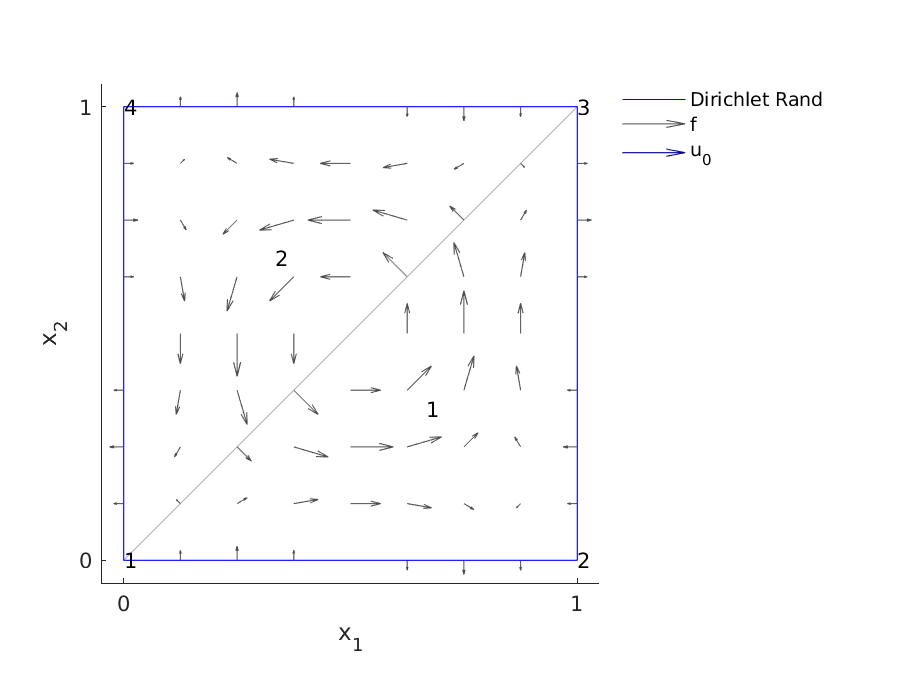
\includegraphics[width=\textwidth]{Plots/SquareBenchmarkInitial3}
	    \caption{Anfangskonfiguration}
	\end{figure}
\end{frame}

\begin{frame}
	\begin{figure}[h]
	    \centering
	    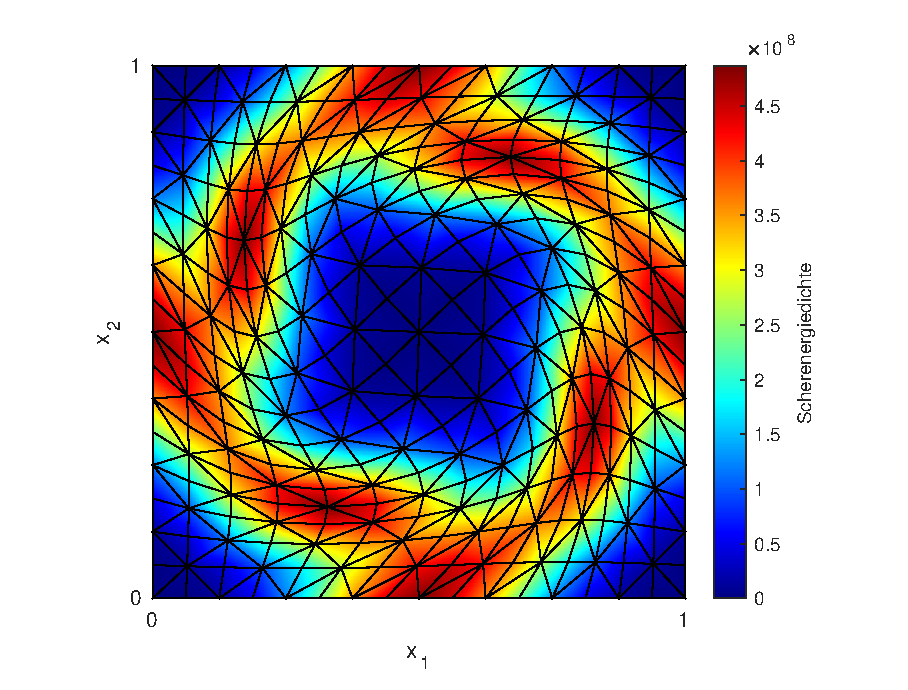
\includegraphics[width=\textwidth]{Plots/SquareBenchmarkDeform5}
	    \caption{Mögliche Deformation des Gebiets.}
	\end{figure}
\end{frame}

\begin{frame}
	\begin{figure}[h]
	    \centering
	    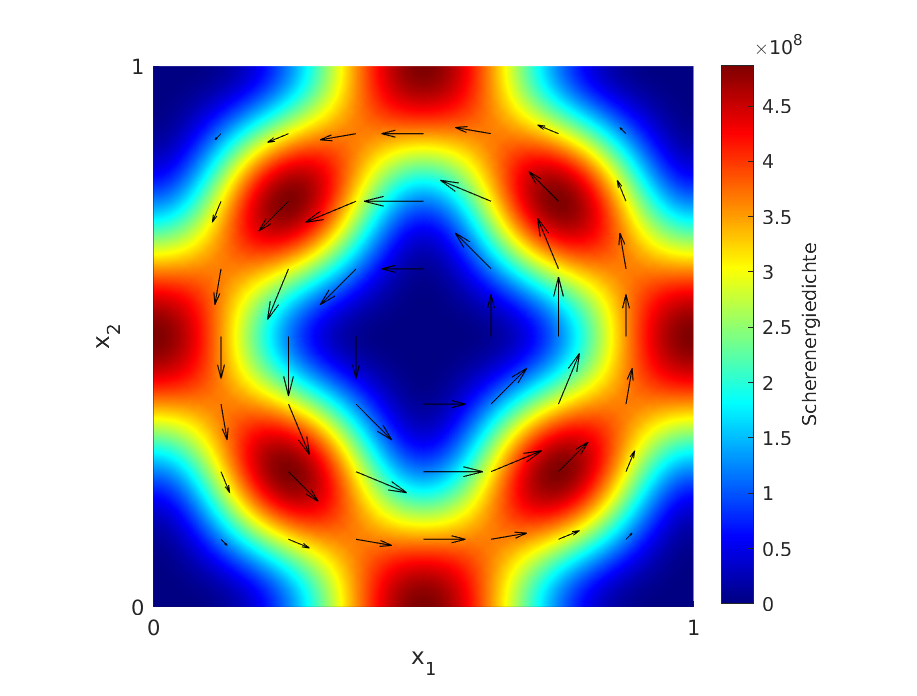
\includegraphics[width=\textwidth]{Plots/SquareBenchmarkSoln3}
	    \caption{Lösung auf dem Gebiet.}
	\end{figure}
\end{frame}

\begin{frame}
	\begin{figure}[h]
	    \centering
	    \scalebox{0.9}{
	    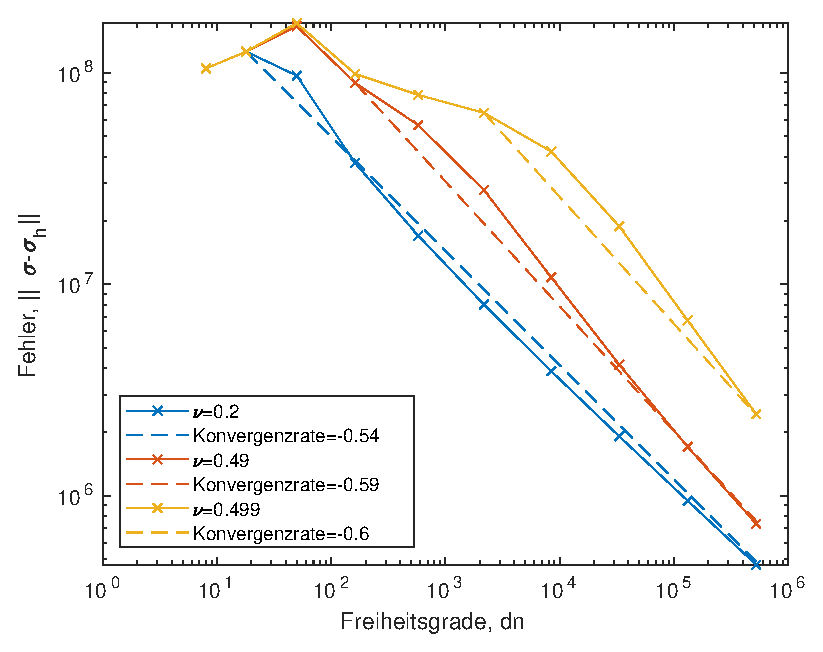
\includegraphics[width=\textwidth]{Plots/SquareBenchmarkNormSigDiff1}
	    }
	    \caption{Fehler}
	\end{figure}
\end{frame}

\begin{frame}
	\begin{figure}[h]
	    \centering
	    \scalebox{0.9}{
	    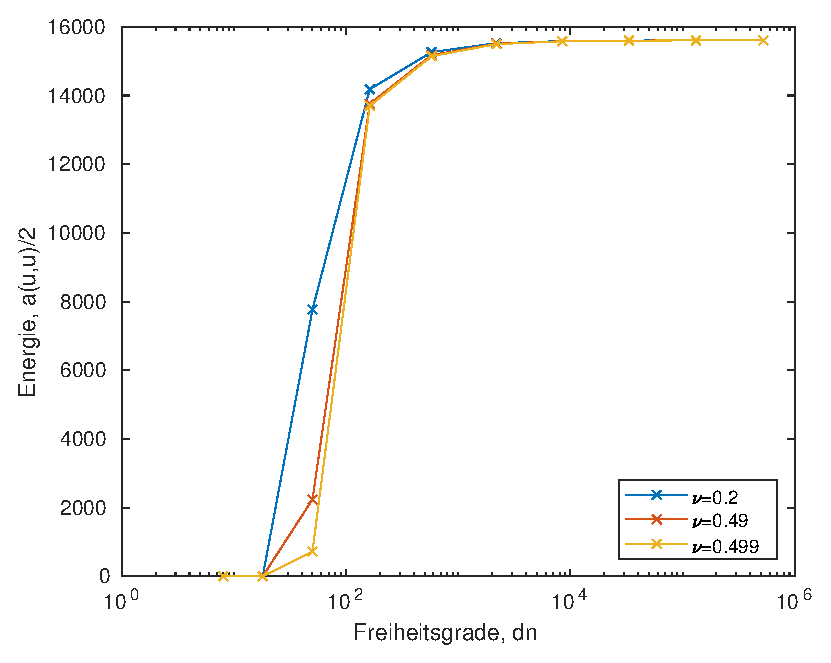
\includegraphics[width=\textwidth]{Plots/SquareBenchmarkTotalEnergy1}
	    }
	    \caption{Energie}
	\end{figure}
\end{frame}

\begin{frame}
	\begin{figure}[h]
	    \centering
	    \scalebox{0.9}{
	    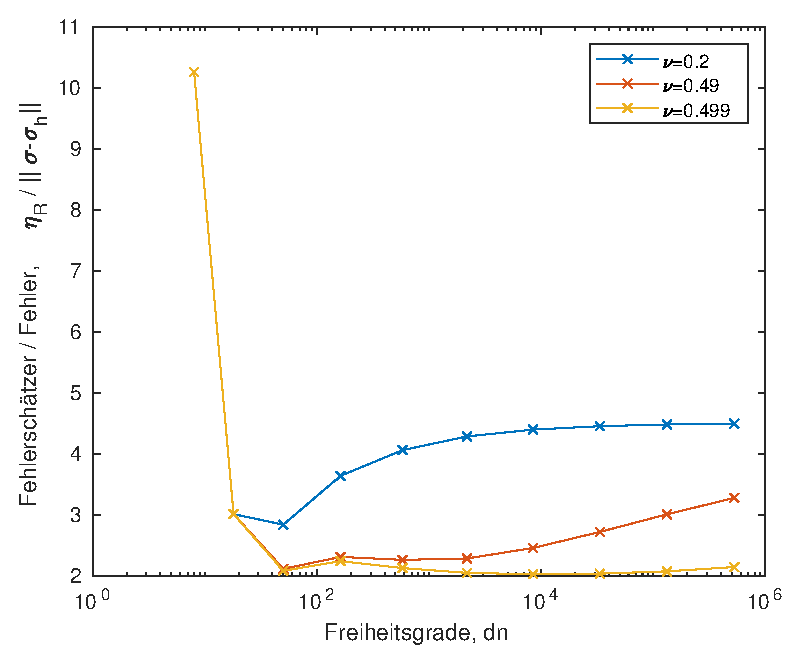
\includegraphics[width=\textwidth]{Plots/SquareBenchmarkEfficiency1}
	    }
	    \caption{Effizienz}
	\end{figure}
\end{frame}

\begin{frame}
	\begin{figure}[h]
	    \centering
	    \scalebox{0.9}{
	    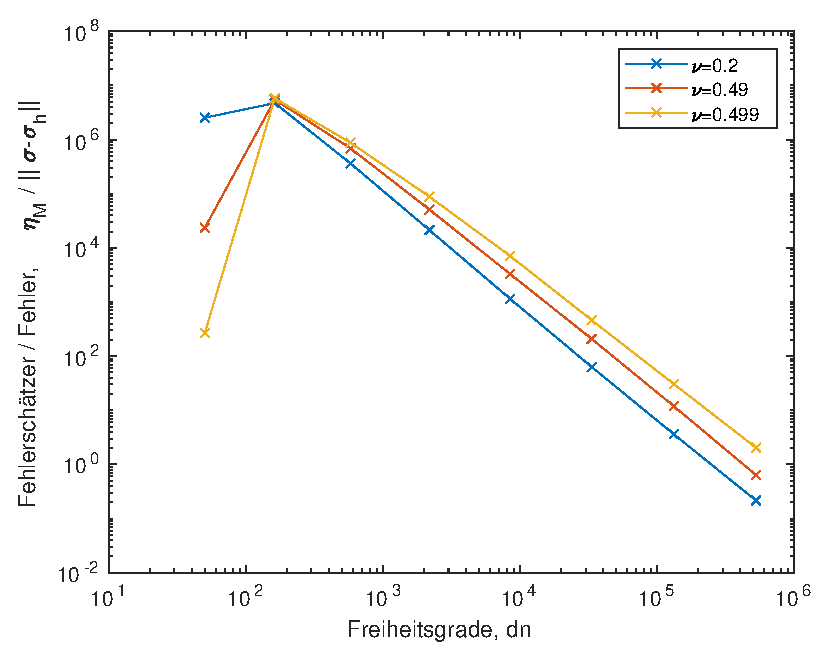
\includegraphics[width=\textwidth]{Plots/SquareBenchmarkInefficiency1}
	    }
	    \caption{Ineffizienz}
	\end{figure}
\end{frame}

\subsection*{Benchmark: L-förmiges Gebiet}
\begin{frame}
	Das Folgende Benchmark stammt aus \cite[Abschnitt 3.4]{Car-2011} und \cite[S.255f.]{Alb-2002}.
	\begin{block}{Benchmark: L-förmiges Gebiet}
	Wir verwenden ein L-förmiges Gebiet und Parameter $\mu=10^7$, $\nu=0.3$ und $\zeta=0.7$. In Polarkoordinaten ist
	\begin{align*}
		u_r(r,\varphi) &= \frac{r^\alpha}{2\mu}\big(-(\alpha+1)\cos\left((\alpha+1)\varphi\right) \\
		&\qquad\qquad+(C_2-\alpha-1)C_1\cos\left((\alpha-1)\varphi\right)\big) \\
		u_\varphi(r,\varphi) &= \frac{r^\alpha}{2\mu}\big((\alpha+1)\sin\left((\alpha+1)\varphi\right) \\
		&\qquad\qquad+(C_2+\alpha-1)C_1\sin\left((\alpha-1)\varphi\right)\big)
	\end{align*}
	mit speziellen Konstanten $C_1$, $C_2$ und $\alpha$ gegeben. Außerdem haben wir $f=0$ und $g=0$.
	\end{block}
\end{frame}


\begin{frame}
	\begin{figure}[h]
	    \centering
	    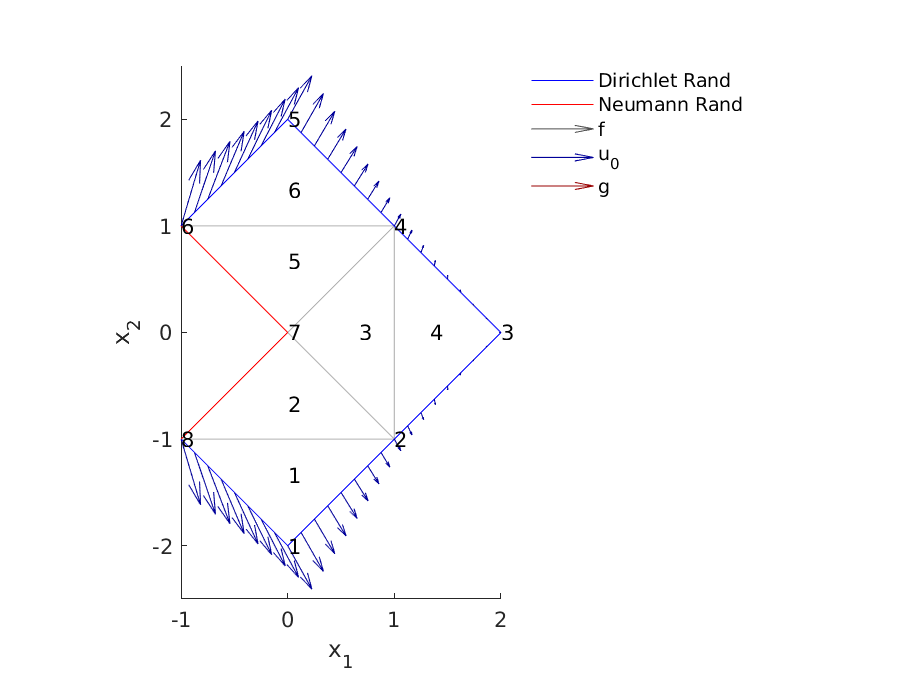
\includegraphics[width=\textwidth]{Plots/LShapeBenchmarkInitial4}
	    \caption{Anfangskonfiguration}
	\end{figure}
\end{frame}

\begin{frame}
	\begin{figure}[h]
	    \centering
	    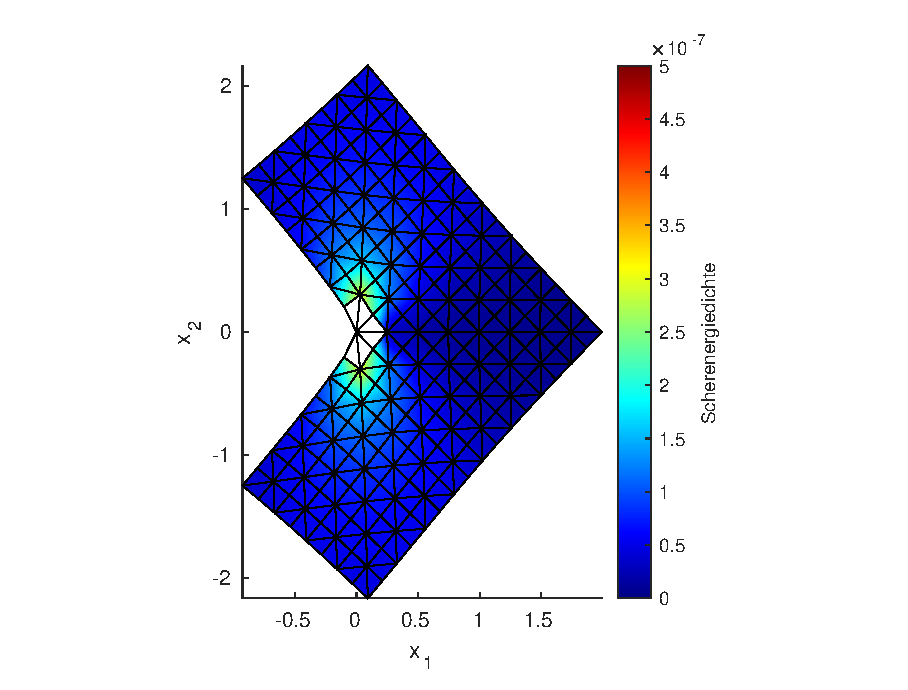
\includegraphics[width=\textwidth]{Plots/LShapeBenchmarkDeform4}
	    \caption{Mögliche Deformation des Gebiets.}
	\end{figure}
\end{frame}

\begin{frame}
	\begin{figure}[h]
	    \centering
	    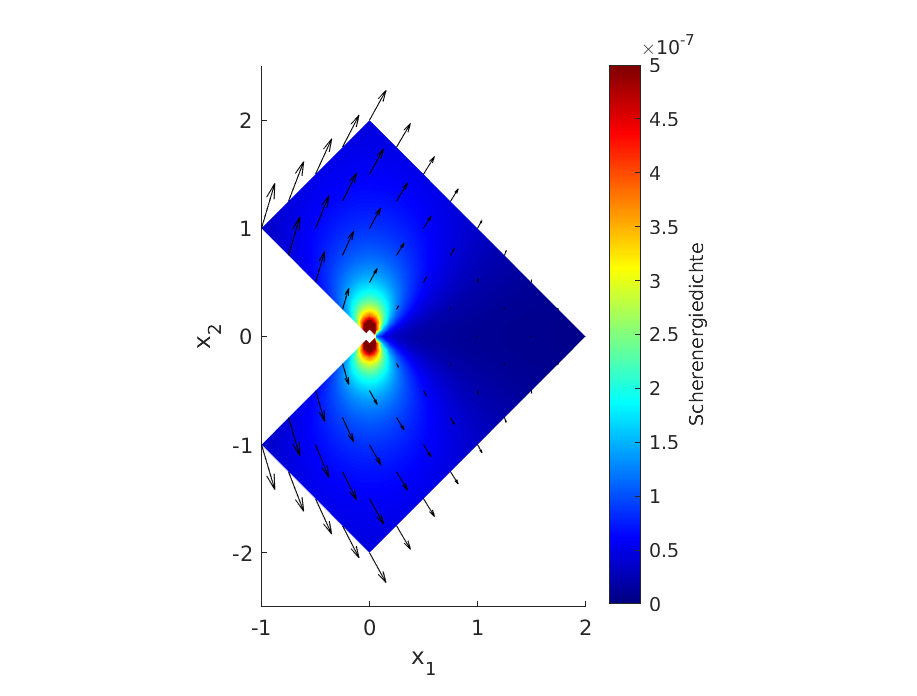
\includegraphics[width=\textwidth]{Plots/LShapeBenchmarkSoln4}
	    \caption{Lösung auf dem Gebiet.}
	\end{figure}
\end{frame}

\begin{frame}
	\begin{figure}[h]
	    \centering
	    \scalebox{0.9}{
	    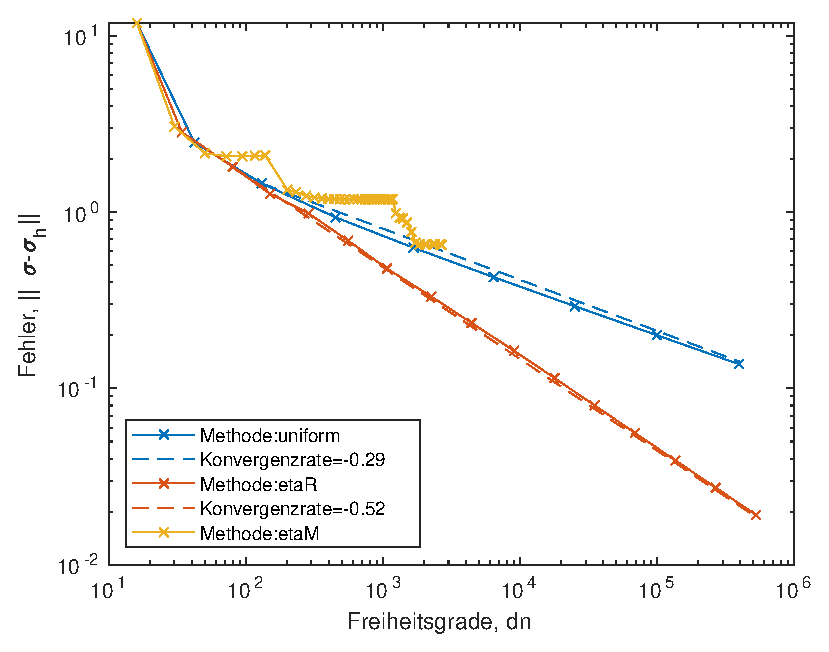
\includegraphics[width=\textwidth]{Plots/AdaptivityBenchmarkNormSigDiff1}
	    }
	    \caption{Fehler}
	\end{figure}
\end{frame}

\begin{frame}
	\begin{figure}[h]
	    \centering
	    \scalebox{0.9}{
	    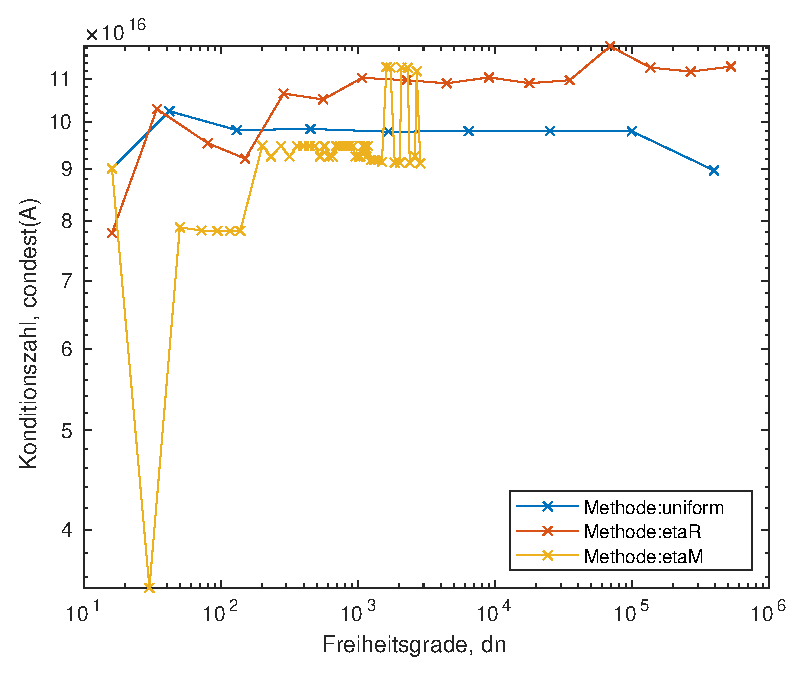
\includegraphics[width=\textwidth]{Plots/AdaptivityBenchmarkCondition1}
	    }
	    \caption{Konditionszahl}
	\end{figure}
\end{frame}

\begin{frame}
	\begin{figure}
	\centering
	\scalebox{0.9}{
	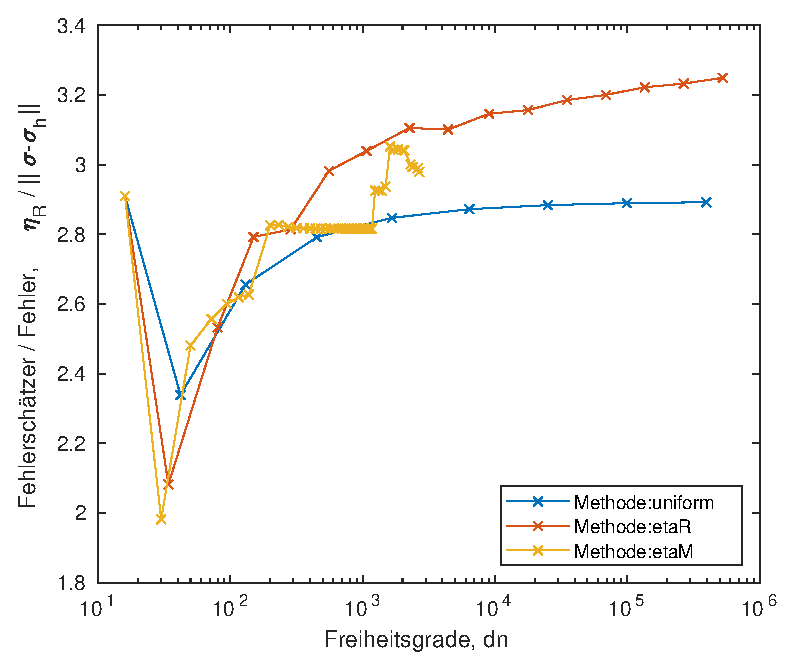
\includegraphics[width=1\textwidth]{Plots/AdaptivityBenchmarkEfficiency1}
	}
	\caption{Effizienz}
	\label{pl:AdaptivityBenchmarkEfficiency}
	\end{figure}
\end{frame}

\begin{frame}
	\begin{figure}
	\centering
	\scalebox{0.9}{
	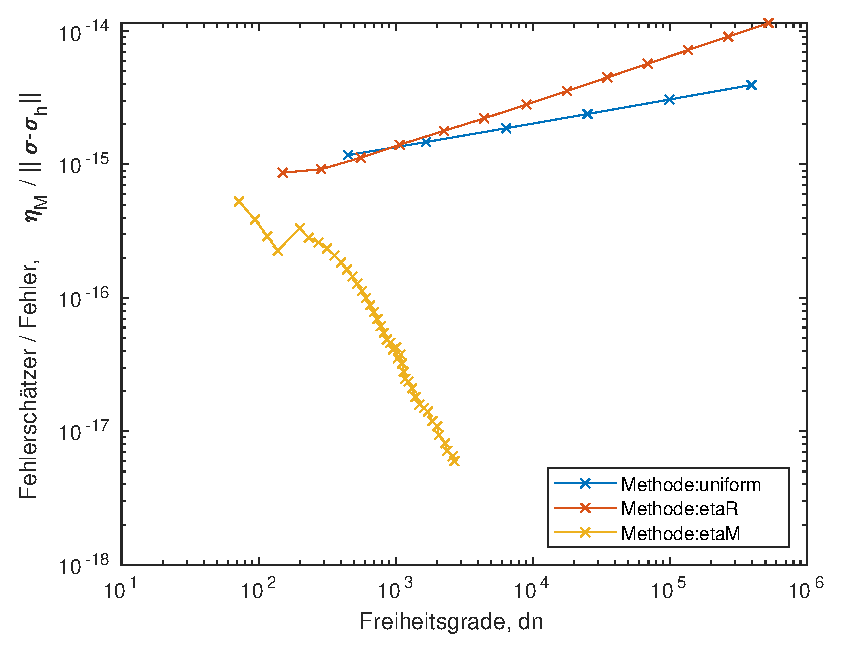
\includegraphics[width=\textwidth]{Plots/AdaptivityBenchmarkInefficiency1}
	}
	\caption{Ineffizienz}
	\label{pl:AdaptivityBenchmarkInefficiency}
	\end{figure}
\end{frame}

\begin{frame}
	\begin{figure}
		\centering
		\begin{subfigure}[b]{0.48\textwidth}
	    \centering
	    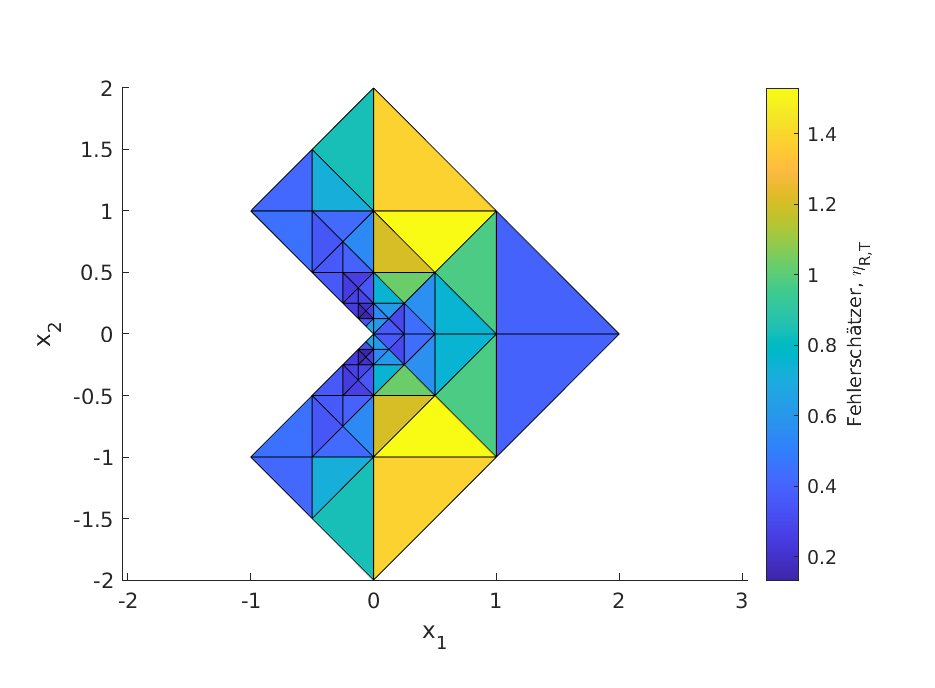
\includegraphics[width=\textwidth]{Plots/LShapeBenchmarkLocaletaR94}
	    \caption{lokaler Fehlerschätzer $\eta_{R,T}$}
	    \end{subfigure}
	    \hfill
	    \begin{subfigure}[b]{0.48\textwidth}
	    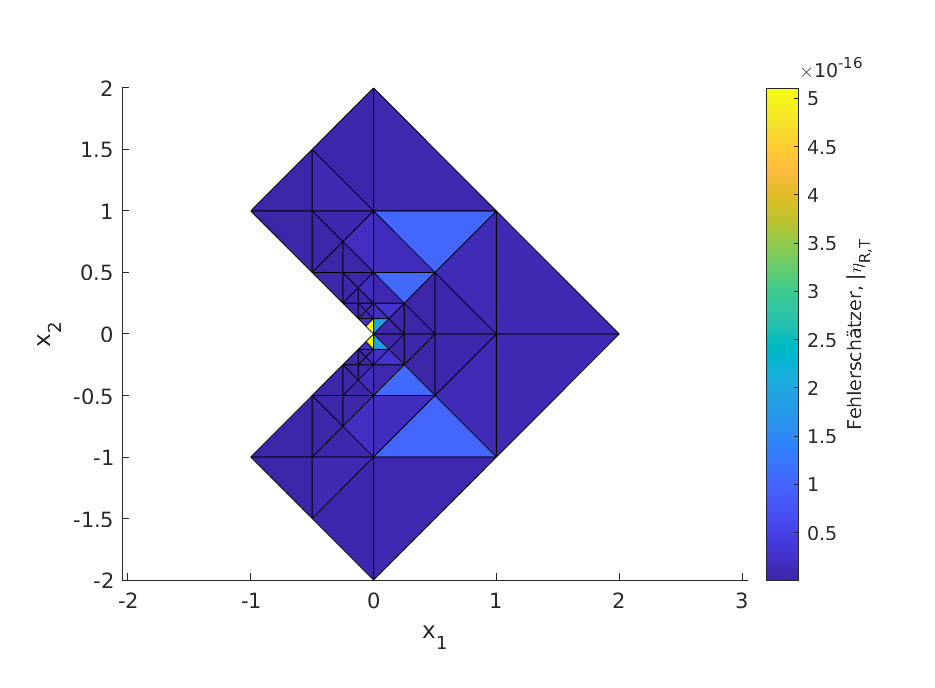
\includegraphics[width=\textwidth]{Plots/LShapeBenchmarkLocaletaM94}
	    \caption{lokaler Fehlerschätzer $\eta_{M,T}$}
	    \end{subfigure}
	    \caption{uniforme Triangulierung bei $d\cdot n=94$.}
	\end{figure}
\end{frame}

\begin{frame}
	\begin{figure}
	\centering
	\begin{minipage}[h]{0.48\textwidth}
	    \centering
	    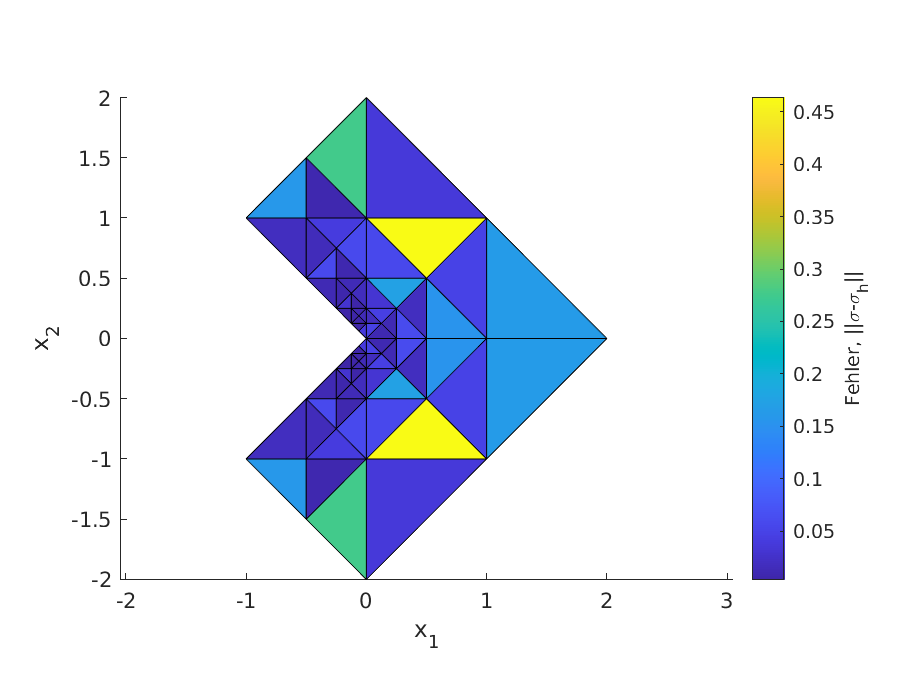
\includegraphics[width=\textwidth]{Plots/LShapeBenchmarkLocalNormSigDiff94}
	    \caption{lokaler Fehler $\norm{\sigma-\sigma_h}$ bei $d\cdot n=94$ Freiheitsgraden.}
	\end{minipage}
	\hfill
	\begin{minipage}[h]{0.48\textwidth}
	    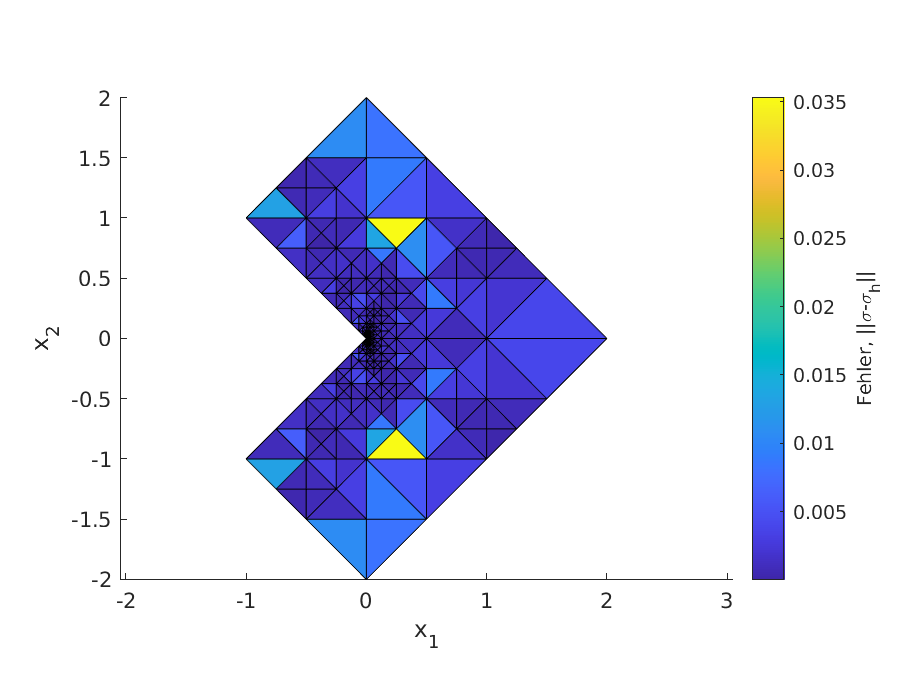
\includegraphics[width=\textwidth]{Plots/LShapeBenchmarkLocalNormSigDiff1610}
	    \caption{lokaler Fehler $\norm{\sigma-\sigma_h}$ bei $d\cdot n=1610$ Freiheitsgraden.}
	\end{minipage}
	\end{figure}
\end{frame}

\begin{frame}
	\begin{figure}
		\centering
		\begin{subfigure}[b]{0.48\textwidth}
	    \centering
	    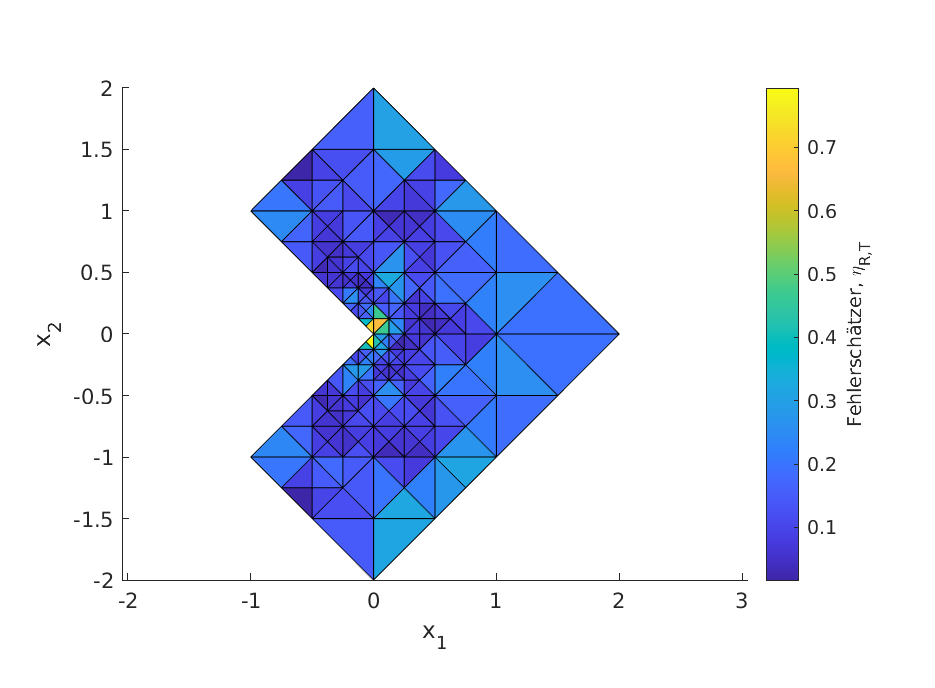
\includegraphics[width=\textwidth]{Plots/LShapeBenchmarkLocaletaR286}
	    \caption{lokaler Fehlerschätzer $\eta_{R,T}$}
	    \end{subfigure}
	    \hfill
	    \begin{subfigure}[b]{0.48\textwidth}
	    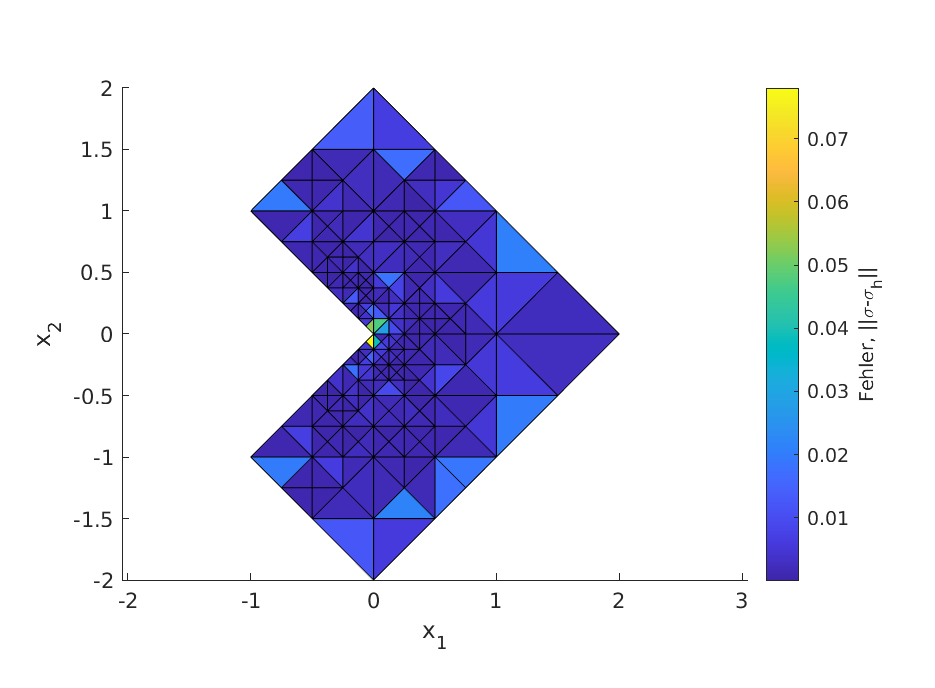
\includegraphics[width=\textwidth]{Plots/LShapeBenchmarkLocalNormSigDiff286}
	    \caption{lokaler Fehler $\norm{\sigma-\sigma_h}$}
	    \end{subfigure}
	    \caption{Adaptive Gitterverfeinerung mit dem residualen Fehlerschätzer $\eta_R$ und $d\cdot n=286$ Freiheitsgraden.}
	\end{figure}
\end{frame}

\section{Zusammenfassung}
\begin{frame}[allowframebreaks]
	\frametitle{Zusammenfassung}
	
	\begin{itemize}
		\item Kontinuierliches Problem: Finde $u\in V$, so dass
		\begin{itemize}
		\item
		Kräftegleichgewicht
		\begin{align*}
			-\int_{\partial\omega}\sigma n\dif s&=\int_\omega f\dif x &&\text{für alle }\omega\subseteq\Omega\text{ regulär genug}\,, \\
			\sigma n&= g &&\text{auf }\Gamma_N\,, \\
			Mu &= w &&\text{auf }\Gamma\,.
		\end{align*}
		\item
		Differenzielles Problem
		\begin{align*}
			\qquad\qquad-\diver\sigma &= f &&\text{auf }\Omega\,,\qquad\qquad\\
			\sigma n &= g &&\text{auf }\Gamma_N\,, \\
			Mu &= w &&\text{auf }\Gamma\,.
		\end{align*}
		\framebreak
		\item
		Variationelles Problem (virtuelle Arbeit)
		\begin{align*}
			a(u,v)&= \ell(v) \qquad &&\text{für alle }v\in V^0\,,\qquad\\
			Mu &= w &&\text{auf }\Gamma\,.
		\end{align*}
		\item
		Optimierungsproblem (Energiefunktional)
		\begin{equation*}
			\begin{aligned}
				u\text{ minimiert }&&  &W=\frac{1}{2}a(\cdot,\cdot)-\ell \\
			\text{unter der Nebenbedingung }&&  &Mu\big\vert_\Gamma = w\big\vert_\Gamma
			\end{aligned}
		\end{equation*}
		\end{itemize}
		\item
		Diskretes Problem: Finde $u_h\in V_h$, so dass
		\begin{align*}
			a(u_h,v_h)&= \ell(v_h) \qquad &&\text{für alle }v_h\in V_h^0\,,\qquad\\
			Mu_h &= w &&\text{auf }\Gamma\,.
		\end{align*}
	\end{itemize}
%	\begin{itemize}
%		\item
%		Implementation als LGS mit Lagrange-Multiplikatoren
%		\begin{align*}
%			\begin{bmatrix}
%				A & B'^\top \\
%				B' & 0
%			\end{bmatrix}
%			\vect{\hu \\ \hp}
%			= \vect{\hl \\ \hw'}
%		\end{align*}
%	\end{itemize}
	
	\begin{itemize}
		\item
		Man zeigt:
		
		
		Kornsche Ungleichung ohne Randbedinungen auf dem Ganzraum $\xrightarrow{\text{Erweiterungsoperator}}$ Kornsche Ungleichung ohne Randbedingungen $\xrightarrow{\text{Starrk"orperbewegungen}}$ Kornsche Ungleichung mit Randbedingungen $\rightarrow$ Positivdefinitheit von $a$
		\item
		Existenz und Eindeutigkeit folgt aus dem Lax-Milgram-Lemma
%		\framebreak
		\item
		Der residuale Fehlerschätzer ist zuverlässig und effizient. Dies sieht man auch in numerischen Experimenten.
		\item
		Der residuale Fehlerschätzer wird verwendet, um das Gitter adaptiv zu verfeinern. Dies verbessert bei manchen Problemen die Konvergenz.
	\end{itemize}
\end{frame}


\section{Quellen}

\begin{frame}[allowframebreaks]
	\frametitle{Quellen}
	\nocite{*}
	\bibliographystyle{plain}
	\setbeamertemplate{bibliography item}[text]
	\bibliography{bibliographyFile}
\end{frame}


\begin{frame}[plain]
	\begin{center}
		\Large{{Danke für die Aufmerksamkeit.}}
	\end{center}
\end{frame}

\frame[plain]

\end{document}
